\documentclass[journal]{IEEEtran}
\usepackage{cite}
\usepackage{amsmath,amssymb}
\usepackage{graphicx}


\usepackage{booktabs}
\usepackage{multirow}
\usepackage{array}
\usepackage{tabularx}
\usepackage{url}
\usepackage{hyperref}
\usepackage{xcolor}

% Algorithms
\usepackage{algorithm}
\usepackage{algpseudocode}

\usepackage{tikz}
\usepackage{comment}
\usetikzlibrary{arrows.meta, positioning}
\hypersetup{hidelinks}

\begin{document}

\title{An Adaptive Physics-Informed Framework for Subsea Pipeline Reliability and Maintenance}

\author{Devesh Shukla, and Vinay Kumar
\thanks{Devesh shukla is with Department of Computer Science and Engineering, IIIT Naya Raipur, 493661 India
(e-mail: devesh253000@iiitnr.edu.in).}
\thanks{Vinay Kumar is with Department of Computer Science and Engineering, IIIT Naya Raipur, 493661 India
(e-mail: vinay@iiitnr.edu.in).}}

\maketitle

\begin{abstract}
Subsea pipelines are exposed to progressive corrosion and discrete
external or operational shocks whose interaction introduces substantial
uncertainty into reliability assessment, remaining useful life (RUL)
prediction, and maintenance planning. Existing stochastic degradation,
competing-failure, and Dynamic Bayesian Network (DBN) approaches address
different aspects of this problem, but degradation modeling, sequential
parameter adaptation, probabilistic prognosis, and maintenance
decision-making are often treated separately. This paper develops an
Adaptive Physics-Informed Dynamic Bayesian Network (API-DBN) that
integrates these functions within a unified condition-updating
framework. Stochastic corrosion is represented by a Wiener process and
shock occurrence by a Poisson process, with a temporally ordered,
state-dependent coupling mechanism describing their interaction.
Sequential Monte Carlo filtering with Markov Chain Monte Carlo
rejuvenation jointly updates the latent degradation state and selected
evolving model parameters as inspection observations become available.
The resulting posterior is propagated through Monte Carlo simulation to
obtain probabilistic RUL estimates, which are subsequently incorporated
into a risk--cost maintenance model. In controlled simulations of
9{,}990 pipelines whose degradation parameters differ between pipelines
and drift over time, API-DBN reduces the RUL mean absolute error by
19\% and the continuous ranked probability score by 29\% relative to a
static-parameter DBN, and its 95\% prediction intervals contain the
true RUL in 95.3\% of forecasts, against 59.9\% for the static DBN.
When each model drives the inspection and replacement decisions for
the same simulated pipelines, the API-DBN-based policy lowers the
expected discounted lifecycle cost by 17\% relative to the
static-DBN-based policy. The benefit of adaptation arises when
degradation parameters vary across assets or over time; with identical,
known parameters a static DBN performs better. Public BSEE/NETL
Gulf of Mexico pipeline and incident records are used to check the
geometry, shock-rate, and failure-cost assumptions.
\end{abstract}



\begin{IEEEkeywords}
Subsea Pipelines, Dynamic Bayesian Networks, Dependent Competing Failures,
Remaining Useful Life, Sequential Monte Carlo, Maintenance Optimization.
\end{IEEEkeywords}
% ============================================================
% I. INTRODUCTION
% ============================================================

\section{Introduction}
\label{sec:introduction}

Subsea pipelines are critical components of offshore energy
infrastructure, transporting hydrocarbons between production
facilities, processing systems, and onshore terminals. Their integrity
is challenged by prolonged exposure to corrosive seawater, high
hydrostatic pressure, operational loading, and accidental external
actions such as dropped objects, anchor interaction, and trawling
\cite{dnvf107}. Historical Gulf of Mexico incident
records further demonstrate that pipeline failures remain an important
integrity-management concern \cite{romeo2024,pfander2024}. Because subsea
inspection, repair, and replacement are costly and operationally
constrained, reliable condition assessment and timely maintenance
planning are essential for managing structural risk over the service
life of these assets.

Subsea pipeline deterioration involves multiple mechanisms whose
effects can coexist and interact. Corrosion produces progressive wall
loss, whereas external or operational shocks can introduce discrete
damage and modify subsequent deterioration. Corrosion-induced wall
thinning can reduce structural resistance to later loading, while
impact-induced damage to protective systems can accelerate subsequent
corrosion. Microbiologically influenced corrosion \cite{yazdi2023} and
fatigue are also important contributors to subsea-pipeline
deterioration; however, the present study focuses
specifically on the dependent interaction between progressive
corrosion and discrete shock-induced damage. Treating these mechanisms
as independent can therefore neglect dependencies that influence
failure probability and remaining useful life (RUL).

Existing integrity-assessment methods address different aspects of
this problem. Deterministic physics-based models provide interpretable
relationships between deterioration and structural capacity but can be
sensitive to parameters established during initial calibration.
Stochastic degradation models, including Wiener and Gamma processes,
represent variability in deterioration evolution
\cite{zhang2018,ling2015}, while dependent competing-failure models
provide mechanisms for representing interactions between degradation
and shocks. Dynamic Bayesian Networks (DBNs) extend probabilistic
reliability assessment across successive time slices and allow uncertain
system states to be updated as evidence becomes available
\cite{straub2009}. DBN applications to subsea pipelines have further
demonstrated the ability to represent degradation, competing-failure
processes, and parameter uncertainty \cite{liu2023,cai2020rul}.
These developments provide important components for condition-based
reliability assessment, but they do not by themselves establish a
complete adaptive prognosis-to-decision framework.

The remaining challenge is primarily one of methodological
integration. Degradation modeling, dependent-failure analysis,
Bayesian state estimation, parameter calibration, RUL prediction, and
maintenance optimization are often addressed as separate stages.
Consequently, new inspection evidence may update an estimate of the
current pipeline condition without consistently revising uncertain
degradation parameters, propagating the resulting posterior uncertainty
to future failure time, and transferring that information to the
maintenance-decision layer. In addition, existing competing-failure
formulations represent several forms of degradation--shock dependence,
including dependence in both directions \cite{sun2021}, but such
coupling has rarely been embedded in a sequentially updated DBN whose
parameters adapt to inspection data. A condition-updating framework is therefore
needed in which inspection evidence jointly informs the evolving
degradation state and selected model parameters, dependent
corrosion--shock behavior is represented explicitly, and the updated
posterior is propagated from reliability assessment to probabilistic
RUL prediction and maintenance planning. Section~\ref{sec:lit}
examines these limitations in detail and establishes the corresponding
research gaps.

To address this problem, this study develops an Adaptive
Physics-Informed Dynamic Bayesian Network (API-DBN) for subsea
pipelines subjected to interacting progressive corrosion and discrete
shocks. Here, ``physics-informed'' refers to embedding stochastic
corrosion kinetics, shock-arrival behavior, state-dependent
corrosion--shock interaction, and a structural failure criterion within
the probabilistic state-transition model. Continuous corrosion is
represented by a Wiener process and shock occurrence by a Poisson
process, with their interaction introduced through a temporally
ordered state-dependent coupling mechanism. The resulting physical
states and uncertain baseline parameters are embedded within a
time-sliced DBN. As inspection observations become available,
Sequential Monte Carlo (SMC) filtering with Metropolis--Hastings MCMC
rejuvenation updates the posterior distribution of the latent
degradation state and selected degradation and shock parameters. This
posterior is subsequently propagated forward by Monte Carlo simulation
to obtain a probabilistic RUL distribution, which is incorporated into
a risk--cost model for inspection and preventive-maintenance planning.

The principal contributions of this study are as follows:
\begin{enumerate}
    \item A physics-informed dependent degradation formulation with a
    continuous parametric corrosion--shock coupling: a sigmoid
    acceleration of the corrosion drift driven by the total equivalent
    damage, and an exponential dependence of the shock intensity on the
    corrosion depth, both acting with temporal ordering across DBN time
    slices.

    \item An adaptive DBN formulation with SMC--MCMC inference that
    sequentially updates the latent degradation state and selected
    evolving baseline parameters as new inspection information becomes
    available, rather than relying exclusively on a single offline
    parameter calibration.

    \item An integrated prognosis-to-decision procedure in which the
    updated posterior distribution is propagated to probabilistic RUL
    and subsequently incorporated into a risk--cost maintenance model
    for selecting inspection intervals and preventive-maintenance
    thresholds.

    \item A controlled simulation study with known failure times in
    which pipelines differ in their degradation parameters, comprising
    matched baselines, a factorial ablation of coupling and MCMC
    rejuvenation, an oracle reference, and a closed-loop evaluation of
    maintenance policies against the simulated truth.
\end{enumerate}

The experimental design deliberately distinguishes controlled
predictive validation from historical application. Quantitative RUL
accuracy is evaluated using controlled simulations for which failure
times are known, whereas the BSEE/NETL records are used to check the
parameter assumptions. The historical records do not provide complete
longitudinal inspection and true-RUL histories for pipeline segments;
consequently, the simulation-based RUL results are not interpreted as
direct historical RUL validation.

The remainder of this paper is organized as follows.
Section~\ref{sec:lit} reviews related work and establishes the research
gap. Section~\ref{sec:overview} presents the problem formulation and
proposed API-DBN methodology, including the dependent degradation
model, sequential Bayesian inference, probabilistic RUL prediction,
and maintenance-decision formulation. Section~\ref{sec:evalsetup}
describes the historical data, controlled simulation design, baselines,
and evaluation protocol. Section~\ref{sec:results} presents and
discusses the predictive, maintenance, and
computational results. Finally, Section~\ref{sec:conclusion}
summarizes the principal findings, limitations, and directions for
future work.

% ============================================================
% END OF SECTION I
% ============================================================
\section{Related Work and Research Gap}
\label{sec:lit}

Research on subsea-pipeline reliability spans stochastic degradation
modeling, competing-failure analysis, probabilistic graphical models,
remaining useful life (RUL) prediction, and maintenance optimization.
These research streams address complementary aspects of integrity
management, but their integration is particularly important when
progressive deterioration and discrete damage events interact and
inspection information becomes available sequentially. This section
reviews the literature from that perspective and identifies the
specific methodological gaps addressed by the proposed API-DBN.


% ------------------------------------------------------------
% II-A
% ------------------------------------------------------------

\subsection{Stochastic Degradation and Dependent Competing-Failure Models}
\label{sec:lit_degradation}

Progressive corrosion is commonly represented using stochastic
degradation processes that account for uncertainty in the evolution of
material loss. Wiener-process formulations are attractive because of
their analytical tractability and ability to represent stochastic
variability in degradation increments \cite{zhang2018}. Gamma-process
models provide an alternative when monotonic degradation is required
\cite{ling2015}. These formulations establish a probabilistic basis for
estimating deterioration and structural reliability, although their
predictive performance depends on how adequately the assumed process
and its parameters represent changing operating and environmental
conditions.

Pipeline reliability is further complicated by the simultaneous
presence of progressive degradation and discrete shocks. Wang
et al.~\cite{wang2011} considered reliability assessment under
degradation and shock processes, while Peng et al.~\cite{peng2010}
developed reliability and maintenance models for systems subject to
multiple dependent competing-failure processes. Such formulations
demonstrate that deterioration and shock mechanisms cannot always be
treated as isolated contributors to system failure.

Subsequent studies have examined more explicit forms of dependence
between the competing mechanisms. Rafiee et al.~\cite{rafiee2014}
modeled dependent competing-failure processes in which shock events can
change the degradation rate, and later generalized the treatment of
competing risks through mixed shock models \cite{rafiee2017}.
Sun et al.~\cite{sun2021} further modeled dependence in both
directions, considering the effect of random shocks on the increments
and rate of a nonlinear Wiener degradation process together with the
effect of degradation on the shock process, and used a time-varying
copula to describe the dependence among failure processes. These approaches provide
an important basis for representing interactions between continuous
deterioration and discrete damage events.

For subsea pipelines the interaction is likewise reciprocal:
accumulated external damage may alter the subsequent corrosion
environment or effective corrosion rate, while progressive wall loss
reduces structural resistance and modifies the effective
susceptibility to later shocks. The present study therefore does not
claim to introduce two-way degradation--shock dependence. Its
distinguishing elements are (i) a specific continuous parametric form
for each direction, namely a sigmoid acceleration of the corrosion
drift driven by the total equivalent damage and an exponential
dependence of the shock intensity on the corrosion depth
(Section~\ref{sec:physics}), and (ii) the embedding of this coupling in
a time-sliced DBN whose latent state and baseline parameters are
updated sequentially from inspection data (Section~\ref{sec:dbn}).




% ------------------------------------------------------------
% II-B
% ------------------------------------------------------------

\subsection{Dynamic Bayesian Reliability and Sequential Updating}
\label{sec:lit_dbn}

Bayesian networks provide a probabilistic representation of conditional
dependencies among uncertain variables, while Dynamic Bayesian Networks
(DBNs) extend this representation across successive time slices.
Straub~\cite{straub2009} demonstrated the use of DBNs for stochastic
deterioration processes, providing a general framework for representing
temporal dependence and updating uncertain system states as evidence
becomes available.

DBN formulations have subsequently been applied to offshore and subsea
reliability problems. Cai et al.~\cite{cai2020resil} developed a
DBN-based resilience-assessment approach for subsea oil and gas
pipelines. More directly related to the present problem, Liu
et al.~\cite{liu2023} considered dependent competing-failure processes
of subsea pipelines under parameter uncertainty using a DBN. These
studies demonstrate the suitability of temporal probabilistic graphical
models for integrating degradation mechanisms, uncertain variables, and
reliability states.

An important distinction, however, exists between updating the
probability distribution of a latent degradation state and allowing the
parameters governing the degradation process to evolve as new evidence
is assimilated. A model may be dynamic at the state level while retaining
parameters obtained through offline calibration. When corrosion rate,
shock frequency, or degradation variability changes over time, updating
the state alone may therefore be insufficient to represent the evolving
condition of the asset.

Sequential Monte Carlo methods provide a natural mechanism for
approximating posterior distributions in nonlinear and non-Gaussian
state-space models. Particle filtering propagates a population of
weighted samples as observations arrive, and Markov chain Monte Carlo
moves applied after resampling (the resample--move algorithm) restore
particle diversity \cite{gilks2001}. Particle methods for joint
inference over latent states and uncertain parameters are reviewed
in \cite{kantas2015}.



The relevant gap is therefore narrower than the absence of dynamic
Bayesian reliability models. DBNs for deterioration and subsea-pipeline
reliability already exist. What remains limited in the literature
reviewed here is the integration of a physics-informed DBN with
sequential joint updating of the latent degradation state and selected
time-evolving baseline degradation parameters as new inspection
observations become available. This distinction motivates the adaptive
DBN and SMC--MCMC formulation presented in
Section~\ref{sec:dbn}.


% ------------------------------------------------------------
% II-C
% ------------------------------------------------------------

\subsection{RUL Prediction and Maintenance Decision Support}
\label{sec:lit_rul}

Reliability assessment and RUL prediction address related but distinct
questions. Reliability characterizes the probability that a system
continues to satisfy its performance requirements over a specified
period, whereas RUL prediction concerns the distribution of the time
remaining before a defined failure condition is reached. For degrading
infrastructure, the latter is particularly useful when inspection and
maintenance decisions must respond to the current estimated condition.

Probabilistic degradation models can be propagated forward to obtain
failure-time or RUL distributions, and competing-failure formulations
have also been linked to maintenance analysis. Peng
et al.~\cite{peng2010}, for example, explicitly considered both
reliability and maintenance for systems subject to dependent competing
failure processes. Risk-based inspection methods have likewise been
developed for corroded subsea pipelines \cite{seo2015}, demonstrating
the importance of connecting deterioration uncertainty with inspection
planning.


The principal issue for the present study is therefore not the absence
of maintenance optimization or RUL methods. Rather, degradation
estimation, probabilistic prognosis, and maintenance optimization are
often treated as distinct stages with different assumptions and
information structures. In such a setting, newly acquired inspection
evidence may update an estimate of current condition without being
propagated consistently through uncertain model parameters, future
failure-time distributions, and the resulting maintenance decision.

This distinction becomes important when maintenance policies are
defined by fixed inspection intervals or deterministic intervention
thresholds. Such policies may not fully exploit changes in the
posterior degradation state or uncertainty revealed by subsequent
inspections. Propagating the updated posterior distribution to RUL and
then incorporating RUL uncertainty into a risk--cost formulation
provides a direct mechanism for linking condition information with
inspection and preventive-maintenance decisions.

Accordingly, the methodological requirement considered in this study is
an inference-to-decision chain in which inspection observations update
the degradation model, the updated posterior is propagated to a
probabilistic failure-time distribution, and that distribution enters
the maintenance objective. Section~\ref{sec:cost} develops this
connection for inspection-interval and preventive-maintenance-threshold
selection.


% ------------------------------------------------------------
% II-D
% ------------------------------------------------------------

\subsection{Research Gap and Positioning of the Present Study}
\label{sec:researchgap}

Table~\ref{tab:comparison} compares representative approaches according
to the methodological capabilities most relevant to the present study.
The comparison is intended to clarify how stochastic degradation,
competing shocks, dependency modeling, dynamic probabilistic inference,
online updating, RUL prediction, and maintenance optimization have been
addressed across the literature. The individual techniques are not
themselves absent from prior work; the principal issue is the extent to
which they are integrated within a common condition-updating framework.

\begin{table*}[t]
\centering
\caption{Methodological Comparison of Representative Approaches Relevant to
Dependent Degradation, Dynamic Reliability Assessment, and Maintenance Planning}
\label{tab:comparison}

\renewcommand{\arraystretch}{1.15}
\setlength{\tabcolsep}{4pt}
\footnotesize

\begin{tabular}{
p{2.5cm}
p{2.0cm}
p{2.1cm}
p{2.0cm}
p{1.7cm}
p{1.6cm}
p{1.5cm}
p{1.8cm}}
\toprule

\textbf{Study} &
\textbf{Degradation Model} &
\textbf{Shock / Competing Failure} &
\textbf{Dependency} &
\textbf{Dynamic Model} &
\textbf{Online Updating} &
\textbf{RUL} &
\textbf{Maintenance} \\

\midrule


Wang et al.~\cite{wang2011} &
Wiener &
Poisson shocks &
Shock$\to$degradation (level or rate) &
No &
No &
No &
No \\


Peng et al.~\cite{peng2010} &
Gamma &
Poisson shocks &
Shock$\to$degradation (abrupt damage) &
No &
No &
No &
Yes \\

Rafiee et al.~\cite{rafiee2014} &
Gamma &
Random shocks &
Rate-dependent &
No &
No &
No &
No \\


Straub~\cite{straub2009} &
General deterioration &
No &
-- &
DBN &
Yes (inspection data) &
No &
No \\


Liu et al.~\cite{liu2023} &
Wiener &
Poisson shocks &
Shock$\to$degradation &
DBN &
Parametric (offline) &
No &
No \\

Cai et al.~\cite{cai2020resil} &
General &
No &
No &
DBN &
No &
No &
No \\


Sun et al.~\cite{sun2021} &
Nonlinear Wiener &
Poisson shocks &
Two-way (copula-based) &
No &
No &
No &
No \\

\textbf{Proposed API-DBN} &
\textbf{Wiener} &
\textbf{Poisson shocks} &
\textbf{Two-way; continuous parametric} &
\textbf{DBN} &
\textbf{SMC--MCMC (state and parameters)} &
\textbf{Probabilistic} &
\textbf{Risk--cost optimization} \\

\bottomrule
\end{tabular}
\end{table*}



The literature synthesis and the comparison in
Table~\ref{tab:comparison} identify four closely related research gaps.

\textit{1) Limited joint state--parameter adaptation.}
Existing stochastic degradation and DBN approaches provide mechanisms
for representing deterioration uncertainty and, in some cases,
updating system states as new information becomes available. However,
the literature reviewed here provides limited integration of online
inspection evidence with joint sequential estimation of the latent
degradation state and selected parameters governing corrosion,
shock occurrence, and process uncertainty. This limitation is
particularly relevant when the underlying degradation environment is
nonstationary and parameters obtained from offline calibration may no
longer adequately represent the current asset condition.

\textit{2) Limited integration of dependent corrosion--shock evolution
within adaptive inference.}
Competing-failure models have established that progressive degradation
and random shocks can be statistically dependent, and dependence in both
directions has been modeled \cite{sun2021}. In the reviewed literature,
however, such dependence is not expressed as a continuous parametric
coupling, in which accumulated shock damage accelerates subsequent
corrosion while the corrosion state modifies the effective shock
intensity, embedded in a sequentially updated DBN. A formulation of
this type must also avoid introducing a directed cycle within a DBN
time slice.

\textit{3) Fragmentation between degradation inference and
probabilistic prognosis.}
Estimating the current degradation state or reliability does not by
itself provide the posterior distribution of the time remaining until
structural failure. For maintenance planning under uncertainty, the
updated state and parameter distributions must be propagated through
the physical failure model to obtain a probabilistic RUL distribution.
The literature reviewed here addresses degradation modeling, Bayesian
reliability assessment, and RUL prediction to different extents, but
their integration within the same adaptive condition-updating chain
remains limited.

\textit{4) Limited integration of updated prognosis with maintenance
decisions.}
Maintenance and risk-based inspection optimization are established
research areas, including formulations for systems subject to dependent
competing failures. The unresolved integration issue is whether a new
inspection observation can propagate consistently from posterior state
and parameter updating to RUL uncertainty and subsequently to a
risk--cost maintenance policy. Without this connection, maintenance
decisions may remain based on fixed schedules, offline parameter
estimates, or prognostic quantities that do not fully reflect the most
recent condition information.

These gaps motivate the API-DBN developed in Section~\ref{sec:overview}.
The proposed framework combines a physics-informed stochastic
degradation model with a temporally ordered corrosion--shock
interaction, sequential SMC--MCMC inference over latent states and
selected evolving baseline parameters, posterior Monte Carlo RUL
prediction, and risk--cost maintenance optimization. The intended
novelty therefore lies primarily in the integration and adaptive
coupling of these elements rather than in claiming that Wiener
degradation, Poisson shocks, DBNs, particle filtering, MCMC, RUL
prediction, or maintenance optimization are individually new.

More specifically, the four gaps established above map directly to the
methodological development in Section~\ref{sec:overview}: the
degradation--failure and corrosion--shock interaction model addresses
the dependent-degradation representation in
Section~\ref{sec:physics}; the adaptive DBN and SMC--MCMC procedure
address joint state--parameter updating in Section~\ref{sec:dbn}; and
posterior forward propagation together with the lifecycle-cost model
connect probabilistic RUL prediction to maintenance decisions in
Section~\ref{sec:cost}. This correspondence provides the basis for the
experimental evaluation in Sections~\ref{sec:evalsetup} and
\ref{sec:results}.

% ============================================================
% END OF SECTION II
% ============================================================


%---------------------------------
% ============================================================
% III. PROBLEM FORMULATION AND PROPOSED API-DBN METHODOLOGY
% ============================================================

\section{Problem Formulation and Proposed API-DBN Methodology}
\label{sec:overview}

The Adaptive Physics-Informed Dynamic Bayesian Network (API-DBN)
integrates stochastic degradation modeling, sequential Bayesian
inference, probabilistic remaining useful life (RUL) prediction, and
maintenance optimization within a unified reliability framework for
subsea pipelines. The modeled degradation state comprises continuous
corrosion damage and cumulative equivalent damage induced by discrete
shocks. Inspection observations are assimilated sequentially to update
both the latent degradation state and selected baseline model
parameters. The resulting posterior distribution is then propagated
forward to characterize uncertainty in future failure time and to
support risk--cost-based inspection and preventive-maintenance
decisions.

Figure~\ref{fig:workflow} summarizes the complete information flow.
Historical pipeline and incident records are first used to check the
parameter assumptions of the degradation and cost models. Continuous corrosion and
discrete shock processes are then embedded within a time-sliced DBN,
where new inspection observations trigger SMC--MCMC updating of the
latent states and adaptive baseline parameters. The updated posterior
is propagated forward through Monte Carlo simulation to obtain a
probabilistic RUL distribution, which subsequently enters the
maintenance-optimization model. Quantitative RUL performance is
evaluated using controlled simulations with known failure times.

\begin{figure}[t]
\centering
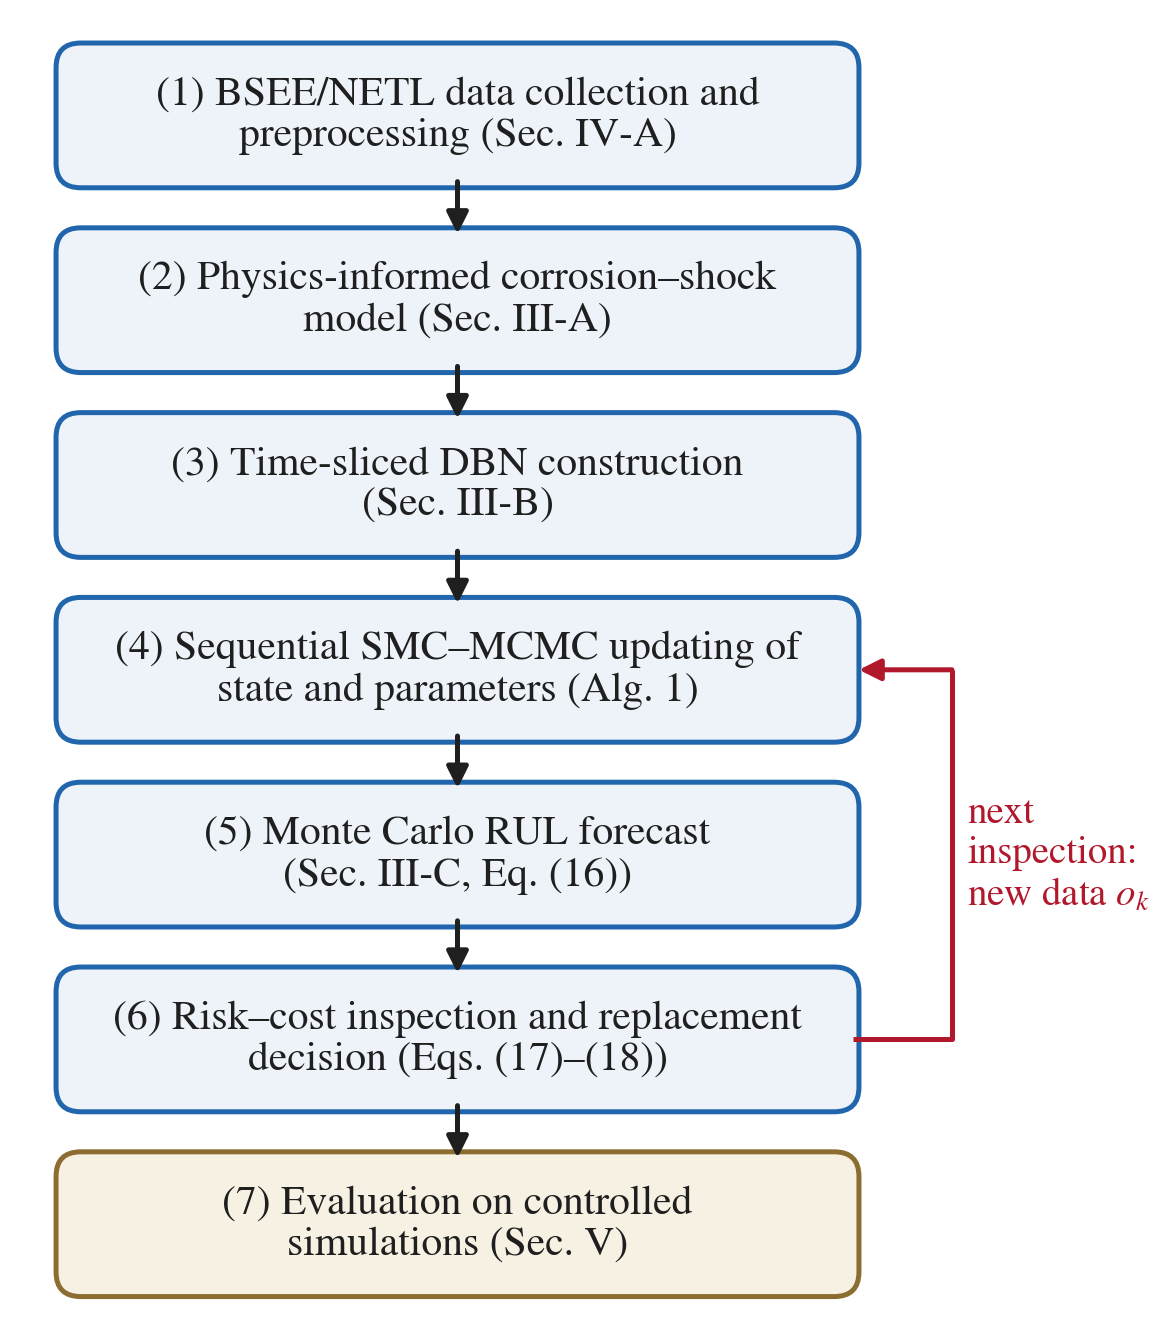
\includegraphics[width=\linewidth]{figures/fig1_workflow.png}
\caption{End-to-end API-DBN workflow. The degradation and failure
model is defined in Section~\ref{sec:physics}, sequential DBN
inference is described in Section~\ref{sec:dbn}, and posterior RUL
prediction and maintenance optimization are formulated in
Section~\ref{sec:cost}. The feedback arrow indicates that the
maintenance decision schedules the next inspection, whose observation
re-enters the DBN and triggers an SMC--MCMC update.}
\label{fig:workflow}
\end{figure}


% ------------------------------------------------------------
% III-A
% ------------------------------------------------------------

\subsection{System Definition and Degradation--Failure Model}
\label{sec:physics}

At inspection epoch $k$, the latent physical state is represented by
$\mathbf{s}_k=(X_k,S_k)$, where $X_k$ denotes corrosion depth and
$S_k$ denotes cumulative equivalent shock damage. The corresponding
total equivalent damage is
$Z_k=X_k+S_k$. The adaptive baseline parameter vector is
$\theta_k=(\mu_k^{(0)},\lambda_k^{(0)},\sigma_{B,k})$, where
$\mu_k^{(0)}$ is the baseline corrosion drift,
$\lambda_k^{(0)}$ is the baseline shock intensity, and
$\sigma_{B,k}$ represents degradation-process uncertainty.
State-dependent effective quantities
$\mu_k^{\mathrm{eff}}$ and $\lambda_k^{\mathrm{eff}}$ govern the
physical propagation of corrosion and shock occurrence, respectively.

Table~\ref{tab:dbnnodes} summarizes the principal variables used in
the API-DBN formulation.

\begin{table}[!ht]
\centering
\caption{DBN Nodes and Descriptions}
\label{tab:dbnnodes}
\begin{tabular}{ll}
\toprule
Node & Description \\
\midrule
$X_k$ & Corrosion depth (continuous, latent) \\
$S_k$ & Cumulative equivalent shock damage (continuous, latent) \\
$\mu_k^{(0)},\mu_k^{\mathrm{eff}}$
& Baseline / effective corrosion drift \\
$\lambda_k^{(0)},\lambda_k^{\mathrm{eff}}$
& Baseline / effective shock intensity \\
$\sigma_{B,k}$ & Diffusion coefficient (time-varying) \\
$Z_k$ & Equivalent total damage ($X_k+S_k$) \\
$F_k$ & Binary failure indicator (Eq.~\eqref{eq:burstfail}) \\
$O_k$ & Observation node (inspection measurement) \\
\bottomrule
\end{tabular}
\end{table}


% ---- Continuous corrosion ----------------------------------

\textit{Continuous corrosion process.}
Wiener processes are widely used for corrosion-depth modeling because
their normally distributed increments provide a tractable
representation of stochastic degradation variability
\cite{zhang2018}. Let $X(t)$ denote the cumulative wall-thinning depth
due to corrosion at time $t$. The corrosion process is modeled as

\begin{equation}
dX(t) = \mu^{\mathrm{eff}}(t,\theta)\,dt
      + \sigma_B\,dB(t),
\label{eq:wiener}
\end{equation}

where $\mu^{\mathrm{eff}}(t,\theta)$ is the time-varying effective
corrosion drift, $\sigma_B$ is the diffusion coefficient, and $B(t)$
is standard Brownian motion.

Unlike a conventional constant-drift formulation
\cite{zhang2018}, the effective drift is allowed to vary through both
the slowly evolving baseline parameter introduced later and the
state-dependent corrosion--shock coupling. Although a Gamma process
guarantees monotonic degradation \cite{ling2015}, the Wiener process
is retained here to represent stochastic variability while maintaining
analytical tractability for sequential filtering.

For a time increment $\Delta t$, the corresponding transition density
is

\begin{equation}
f_X(x_k \mid x_{k-1}) =
\frac{1}{\sqrt{2\pi\sigma_B^2\Delta t}}
\exp\!\left(
-\frac{
(x_k-x_{k-1}-\mu^{\mathrm{eff}}_{k}\Delta t)^2
}{
2\sigma_B^2\Delta t
}
\right).
\label{eq:transdens}
\end{equation}

Equation~\eqref{eq:transdens} assumes a constant effective drift over
each interval $\Delta t$, whereas the baseline drift
$\mu^{(0)}$ may evolve across successive inspection epochs. Independent
increments are assumed. This formulation can produce non-physical
negative increments at the latent-state level, which remains a
limitation relative to strictly monotonic Gamma-process formulations.
Process uncertainty and inspection uncertainty are treated separately:
$\sigma_B$ governs physical state-process variability, whereas the
observation-noise variance introduced in Section~\ref{sec:dbn}
represents measurement uncertainty.


% ---- Shock process -----------------------------------------

\textit{Discrete shock process and equivalent damage.}
Operational and environmental impacts are represented as random shock
events using a time-varying Poisson process
\cite{rafiee2017}. For the interval $(t_{k-1},t_k]$, the number of
shock arrivals satisfies

\begin{equation}
N_k-N_{k-1}
\sim
\mathrm{Poisson}\!\left(
\int_{t_{k-1}}^{t_k}
\lambda^{\mathrm{eff}}(u)\,du
\right).
\label{eq:poisson}
\end{equation}

The Poisson formulation provides a tractable representation of random
shock occurrence while allowing the effective arrival intensity
$\lambda^{\mathrm{eff}}$ to vary with the degradation state. Arrivals
are therefore conditionally independent given the intensity path
$\{\lambda^{\mathrm{eff}}(u)\}$, but not unconditionally independent,
because $\lambda^{\mathrm{eff}}$ itself depends on the evolving
degradation state (Eq.~\eqref{eq:lambdaeff}). Shock magnitudes are
independent and identically distributed and independent of the arrival
times.

Each shock has a physical magnitude $Y_i$, such as dent depth or
impact energy. In the spirit of the cumulative-damage shock models of
\cite{rafiee2017}, the shock is mapped to an equivalent wall-loss
increment through the power law

\begin{equation}
\Delta S_i = \kappa\,Y_i^{\eta},
\label{eq:shockmap}
\end{equation}

where $Y_i\sim\mathcal{N}(\mu_{y_0},\sigma_{y_0}^2)$, truncated at zero,
and $\kappa$ and $\eta$ are material- and geometry-dependent
coefficients. With the values in Table~\ref{tab:simparams}, the mean
equivalent wall loss per shock is
$\mathbb{E}[\Delta S_i]=\kappa\,\mathbb{E}[Y_i^{\eta}]\approx0.17$~mm.
The cumulative equivalent shock damage is

\[
S(t)=\sum_{i:t_i\le t}\Delta S_i .
\]

The power-law form of Eq.~\eqref{eq:shockmap} is a modelling
assumption of this study, and
its coefficients require empirical calibration for a specific asset
class, which is an important limitation of this representation.


% ---- Coupling ----------------------------------------------

\textit{State-dependent corrosion--shock coupling.}
Existing step-change formulations can represent a shock-induced change
in degradation rate through abrupt transitions
\cite{rafiee2014,sun2021}. The present framework instead uses a
continuous sigmoid relationship. Let $\mu_k^{(0)}$ denote the baseline
corrosion drift estimated sequentially and
$\mu_k^{\mathrm{eff}}$ the corresponding effective corrosion rate
after accounting for accumulated damage:

\begin{equation}
\mu^{\mathrm{eff}}_k =
\mu^{(0)}_k
\left[
1+(\alpha-1)
\cdot
\frac{1}{
1+\exp[-r_s(Z_{k-1}-W_0)]
}
\right],
\label{eq:mueff}
\end{equation}

where $Z_{k-1}=X_{k-1}+S_{k-1}$ is the total equivalent damage,
$W_0$ is the midpoint of the sigmoid transition, $\alpha$ is the
asymptotic acceleration factor, and $r_s$ (mm$^{-1}$) is the steepness
of the transition. At zero damage the factor equals
$1+(\alpha-1)/(1+e^{r_sW_0})=1.38$ for the values in
Table~\ref{tab:simparams}, so $\mu_k^{(0)}$ is a baseline parameter
rather than the initial effective drift, and the transition spans
about $2\ln 9/r_s=8.8$~mm between 10\% and 90\% of the full
acceleration. The relationship thus provides a gradual, continuous
increase of the corrosion rate with accumulated damage, avoiding the
discontinuity associated with a step-function representation.

The reverse dependency is introduced by allowing the effective shock
arrival intensity to depend on the current corrosion state:

\begin{equation}
\lambda^{\mathrm{eff}}_k =
\lambda^{(0)}_k
\exp\!\left(
\gamma_1 X_{k-1}+\gamma_2 E_k
\right),
\label{eq:lambdaeff}
\end{equation}

where $\lambda_k^{(0)}$ denotes the sequentially updated baseline
shock intensity, $\gamma_1$ (mm$^{-1}$) sets the sensitivity of the
shock intensity to the corrosion depth, and $E_k$ is an optional
standardized environmental covariate (e.g., wave height or current
speed) with coefficient $\gamma_2$. No environmental covariate is used
in the experiments reported here ($E_k=0$), so the effective shock
intensity depends on the corrosion depth only; $\gamma_1$ is given in
Table~\ref{tab:simparams}.

Equations~\eqref{eq:mueff}--\eqref{eq:lambdaeff} therefore establish
a temporally two-way, state-dependent interaction: accumulated shock
damage contributes to acceleration of the corrosion process, whereas
the corrosion state modifies the effective shock intensity. Both
dependencies act with temporal ordering across successive DBN time
slices, avoiding a directed cycle within an individual time slice.


% ---- Failure criterion -------------------------------------

\textit{Structural failure criterion.}
The corrosion and equivalent shock-damage channels are combined
through a simplified burst-pressure formulation adapted from
DNV-RP-F101 \cite{dnv2017}:

\begin{equation}
P_{\mathrm{burst}}(t) =
\frac{2\,t_{\mathrm{nom}}\,\mathrm{SMYS}}
     {D-t_{\mathrm{nom}}}
\cdot
\frac{
1-d(t)/t_{\mathrm{nom}}
}{
1-d(t)/(t_{\mathrm{nom}}M)
},
\label{eq:burst}
\end{equation}

where

\[
d(t)=X(t)+S(t)
\]

is the effective defect depth and

\begin{equation}
M =
\sqrt{
1+0.8\,\frac{L^2}{D\,t_{\mathrm{nom}}}
}
\label{eq:folias}
\end{equation}

is the Folias bulging factor. Here, $L$ is the defect length, $D$ is
the pipe diameter, and $t_{\mathrm{nom}}$ is the nominal wall
thickness. Unlike the recommended practice, which uses the specified
minimum tensile strength and a length-correction factor with
coefficient 0.31, Eqs.~\eqref{eq:burst}--\eqref{eq:folias} use SMYS and
the Folias factor with coefficient 0.8, both of which lower the
predicted burst pressure.

Structural failure in the API-DBN is defined by

\begin{equation}
P_{\mathrm{burst}}(t)
\le
P_{\mathrm{op}}(t),
\label{eq:burstfail}
\end{equation}

Because $P_{\mathrm{burst}}$ decreases monotonically with $d$,
Eq.~\eqref{eq:burstfail} is equivalent to $Z\ge d_{\mathrm{crit}}$,
where $d_{\mathrm{crit}}=12.07$~mm (63\% of the wall) for the case in
Table~\ref{tab:simparams}; a single large shock that carries $Z$ past
$d_{\mathrm{crit}}$ therefore causes immediate failure. No separate
adaptive degradation threshold is propagated as an inference
parameter. Defect geometry is simplified, and additional failure
mechanisms such as girth-weld cracking are not explicitly represented
in the present model.


% ------------------------------------------------------------
% III-B
% ------------------------------------------------------------

\subsection{Adaptive DBN Formulation and Online Bayesian Updating}
\label{sec:dbn}

The physical degradation model defined above is embedded in a
time-sliced Dynamic Bayesian Network so that uncertain degradation
states and selected model parameters can be updated when new inspection
information becomes available. Each DBN slice spans one inspection
interval $(t_{k-1},t_k]$, $k=1,\dots,N_I$. Within a slice the state is
propagated in sub-steps of length $\Delta t$ using
Eqs.~\eqref{eq:transdens}--\eqref{eq:lambdaeff}, with the effective
rates re-evaluated at every sub-step from the current state, whereas
the baseline parameters change only between slices.


% ---- Observation model -------------------------------------

\textit{Observation model.}
Inspection measurements are related explicitly to the latent
degradation state rather than being incorporated into the
state-transition noise. When an inspection reports total equivalent
degradation,

\begin{equation}
O_k=X_k+S_k+v_k,
\qquad
v_k\sim\mathcal{N}(0,\sigma_v^2),
\label{eq:obs}
\end{equation}

where $\sigma_v^2$ denotes the inspection-error variance reported in
Table~\ref{tab:simparams}. If an inspection technology reports
corrosion depth alone, the reduced observation model
$O_k=X_k+v_k$ can be used. Equation~\eqref{eq:obs} is used in the
reported experiments and yields the particle-filter likelihood

\[
p(O_k\mid\mathbf{s}_k)
=
\mathcal{N}
\left(
O_k;
X_k+S_k,
\sigma_v^2
\right).
\]


% ---- DBN formulation ---------------------------------------

\textit{Temporal DBN formulation.}
Time-sliced conditional dependencies follow the standard DBN
representation \cite{straub2009}. The joint distribution is written as

\begin{equation}
p(\mathbf{s}_{0:N_I},\theta_{0:N_I},o_{1:N_I})
=
p(\mathbf{s}_0)\,p(\theta_0)
\prod_{k=1}^{N_I}
p(o_k\mid\mathbf{s}_k)\,
p(\mathbf{s}_k\mid\mathbf{s}_{k-1},\theta_k)\,
p(\theta_k\mid\theta_{k-1}),
\label{eq:factorization}
\end{equation}

where $p(\mathbf{s}_0)$ and $p(\theta_0)$ are the initial distributions
of Algorithm~\ref{alg:smc}, $p(o_k\mid\mathbf{s}_k)$ is the observation
likelihood in Eq.~\eqref{eq:obs},
$p(\mathbf{s}_k\mid\mathbf{s}_{k-1},\theta_k)$ represents the
physics-informed state transition induced by
Eqs.~\eqref{eq:wiener}--\eqref{eq:shockmap} together with the
coupling in Eqs.~\eqref{eq:mueff}--\eqref{eq:lambdaeff}, and
$p(\theta_k\mid\theta_{k-1})$ describes the sequential evolution of
the adaptive baseline parameters. Within each slice the parameters are
propagated first and the state then moves from $\mathbf{s}_{k-1}$ to
$\mathbf{s}_k$ under $\theta_k$, which is the order used in
Algorithm~\ref{alg:smc}.

Figure~\ref{fig:slices} shows two consecutive DBN time slices. Solid
arcs represent the state, parameter, and observation dependencies,
whereas the dashed arcs denote the temporally ordered corrosion--shock
coupling of Eqs.~\eqref{eq:mueff}--\eqref{eq:lambdaeff}: the total
damage $Z_k$ affects the corrosion increment of the next slice, and the
corrosion depth $X_k$ affects its shock intensity. Every arc points
within a slice or forward in time, so the unrolled network is a
directed acyclic graph.

\begin{figure}[t]
\centering
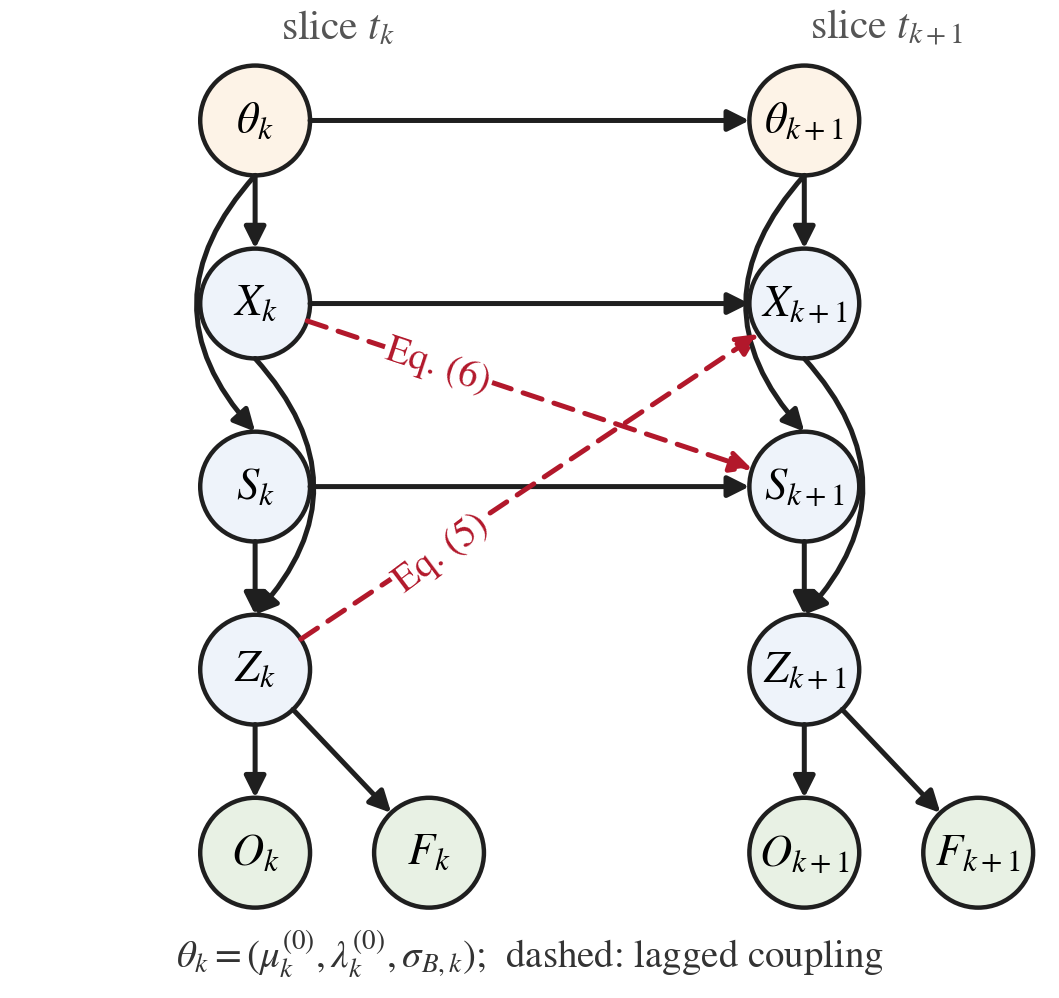
\includegraphics[width=0.9\linewidth]{figures/fig2_dbn.png}
\caption{Two-slice representation of the API-DBN, with
$\theta_k=(\mu_k^{(0)},\lambda_k^{(0)},\sigma_{B,k})$. Solid arrows
denote parameter, state, and observation dependencies; dashed arrows
denote the lagged corrosion--shock coupling of
Eqs.~\eqref{eq:mueff}--\eqref{eq:lambdaeff}. All arrows point within a
slice or forward in time, so the graph is acyclic.}
\label{fig:slices}
\end{figure}


% ---- Adaptive parameter evolution --------------------------

\textit{Adaptive parameter evolution.}
\label{sec:transitions}

The baseline parameters are constrained to remain positive while
being allowed to adapt gradually as additional evidence becomes
available. Following the random-walk (artificial-dynamics) approach to
parameter tracking in particle methods \cite{kantas2015}, the baseline
parameters evolve between slices as

\begin{equation}
\log \mu_k^{(0)}
=
\log \mu_{k-1}^{(0)}
+
\eta_{\mu,k},
\qquad
\eta_{\mu,k}\sim
\mathcal{N}(0,\sigma_\mu^2),
\label{eq:muwalk}
\end{equation}

\begin{equation}
\log \lambda_k^{(0)}
=
\log \lambda_{k-1}^{(0)}
+
\eta_{\lambda,k},
\qquad
\eta_{\lambda,k}\sim
\mathcal{N}(0,\sigma_\lambda^2),
\label{eq:lambdawalk}
\end{equation}

and

\begin{equation}
\log \sigma_{B,k}
=
\log \sigma_{B,k-1}
+
\eta_{\sigma,k},
\qquad
\eta_{\sigma,k}\sim
\mathcal{N}(0,\sigma_{\sigma}^2).
\label{eq:sigmaBwalk}
\end{equation}

The effective operating quantities
$\mu_k^{\mathrm{eff}}$ and $\lambda_k^{\mathrm{eff}}$ are subsequently
obtained from the baseline parameters through
Eqs.~\eqref{eq:mueff}--\eqref{eq:lambdaeff}. Thus, the stochastic
random walks describe gradual evolution of the baseline parameters,
whereas the effective parameters represent deterministic
state-dependent transformations used in the physical propagation
model.

Parameter evolution is assumed Markovian, with no explicit coupling
among the random-walk innovations of the different baseline
parameters. The standard deviations $\sigma_\mu$, $\sigma_\lambda$, and
$\sigma_\sigma$ are specified per year; for a slice of $\Delta_k$ years
they are multiplied by $\sqrt{\Delta_k}$. Structural failure remains governed solely by
Eq.~\eqref{eq:burstfail}; no adaptive failure-threshold parameter is
introduced.


% ---- SMC-MCMC inference ------------------------------------

\textit{Sequential SMC--MCMC inference.}
\label{sec:smc}

The filtering distribution is approximated using $M$ particles within
a bootstrap particle filter augmented by Metropolis--Hastings MCMC
rejuvenation. When the effective sample size falls below $M/2$, the
particles are resampled systematically, and each resampled particle
then receives Metropolis--Hastings moves on its current parameters to
reduce particle impoverishment \cite{gilks2001}.

With the state path held fixed, the move targets
$p(\theta_k\mid\theta_{k-1},\mathbf{s}_{k-1},\mathbf{s}_k)\propto
p(\mathbf{s}_k\mid\mathbf{s}_{k-1},\theta_k)\,p(\theta_k\mid\theta_{k-1})$,
so that a proposal $\theta^*$ is accepted with probability

\begin{equation}
\beta =
\min\!\left(
1,\,
\frac{
p(\mathbf{s}_k\mid\mathbf{s}_{k-1},\theta^*)\,
p(\theta^*\mid\theta_{k-1})
}{
p(\mathbf{s}_k\mid\mathbf{s}_{k-1},\theta)\,
p(\theta\mid\theta_{k-1})
}
\right).
\label{eq:mh}
\end{equation}

The observation likelihood does not depend on $\theta_k$ once the state
is fixed and therefore cancels. Because the corrosion increments are
Gaussian and the shock counts Poisson given the effective rates,
$p(\mathbf{s}_k\mid\mathbf{s}_{k-1},\theta)$ is available in closed form
from each particle's sub-step path. Proposals are Gaussian random walks
on $\log\theta_k$ whose standard deviations equal those of the
parameter random walk for the slice; five sweeps are applied after each
resampling step, and the mean acceptance rate in the reported
experiments is 44\%. No bounds are imposed after initialization,
because the logarithmic parameterization keeps all parameters positive.
Algorithm~\ref{alg:smc} summarizes the complete procedure.

\begin{algorithm}[t]
\caption{Sequential Monte Carlo with MCMC Rejuvenation}
\label{alg:smc}
\begin{algorithmic}[1]

\Require Observation likelihood Eq.~\eqref{eq:obs}; number of
particles $M$; resampling threshold $M/2$

\State \textbf{Initialization:}
for $m=1,\dots,M$, set $\mathbf{s}_0^{(m)}=(0,0)$ and draw the baseline
parameters from their priors:
$\mu_0^{(0)}\sim U(0.2,0.8)$~mm/yr,
$\lambda_0^{(0)}\sim\mathrm{Gamma}(\text{shape }2,\ \text{scale }0.4)$
truncated to $[0.2,5]$~yr$^{-1}$,
$\sigma_{B,0}\sim U(0.1,0.3)$.
Set weights $w_0^{(m)}=1/M$.

\For{$k=1$ to $N_I$}

    \State \textbf{Parameter evolution:}
    for each $m$, propagate
    $\mu_k^{(0),(m)}$,
    $\lambda_k^{(0),(m)}$, and
    $\sigma_{B,k}^{(m)}$
    according to
    Eqs.~\eqref{eq:muwalk}--\eqref{eq:sigmaBwalk}.

    \State \textbf{Propagation:}
    for each $m$ and each sub-step of the slice, compute
    $\mu^{\mathrm{eff},(m)}$ and $\lambda^{\mathrm{eff},(m)}$ from
    $\theta_k^{(m)}$ and the current state using
    Eqs.~\eqref{eq:mueff}--\eqref{eq:lambdaeff}, sample the corrosion
    increment from Eq.~\eqref{eq:transdens} and the shock count from
    $\mathrm{Poisson}(\lambda^{\mathrm{eff},(m)}\Delta t)$, and
    accumulate shock damage via Eq.~\eqref{eq:shockmap}.

    \If{observation $o_k$ available}

        \State \textbf{Weighting:}
        $w_k^{(m)}
        \propto
        w_{k-1}^{(m)}
        p(o_k\mid x_k^{(m)},s_k^{(m)})$
        via Eq.~\eqref{eq:obs}; particles whose path reached
        $d_{\mathrm{crit}}$ during the slice receive zero weight, because
        the pipeline was found intact; normalize.

        \State \textbf{Resampling:}
        compute
        $\mathrm{ESS}
        =
        1/\sum_m(w_k^{(m)})^2$;
        if $\mathrm{ESS}<M/2$, resample systematically.

        \State \textbf{MCMC rejuvenation:}
        after resampling, apply five Metropolis--Hastings sweeps to each
        particle's $\theta_k$ with acceptance probability $\beta$ from
        Eq.~\eqref{eq:mh}.

    \EndIf

\EndFor

\end{algorithmic}
\end{algorithm}

Figure~\ref{fig:flow} provides the corresponding algorithmic flow.
The posterior particle population resulting from the sequential
updating stage forms the starting distribution for the RUL prediction
and maintenance-decision model developed in
Section~\ref{sec:cost}.

\begin{figure}[t]
\centering
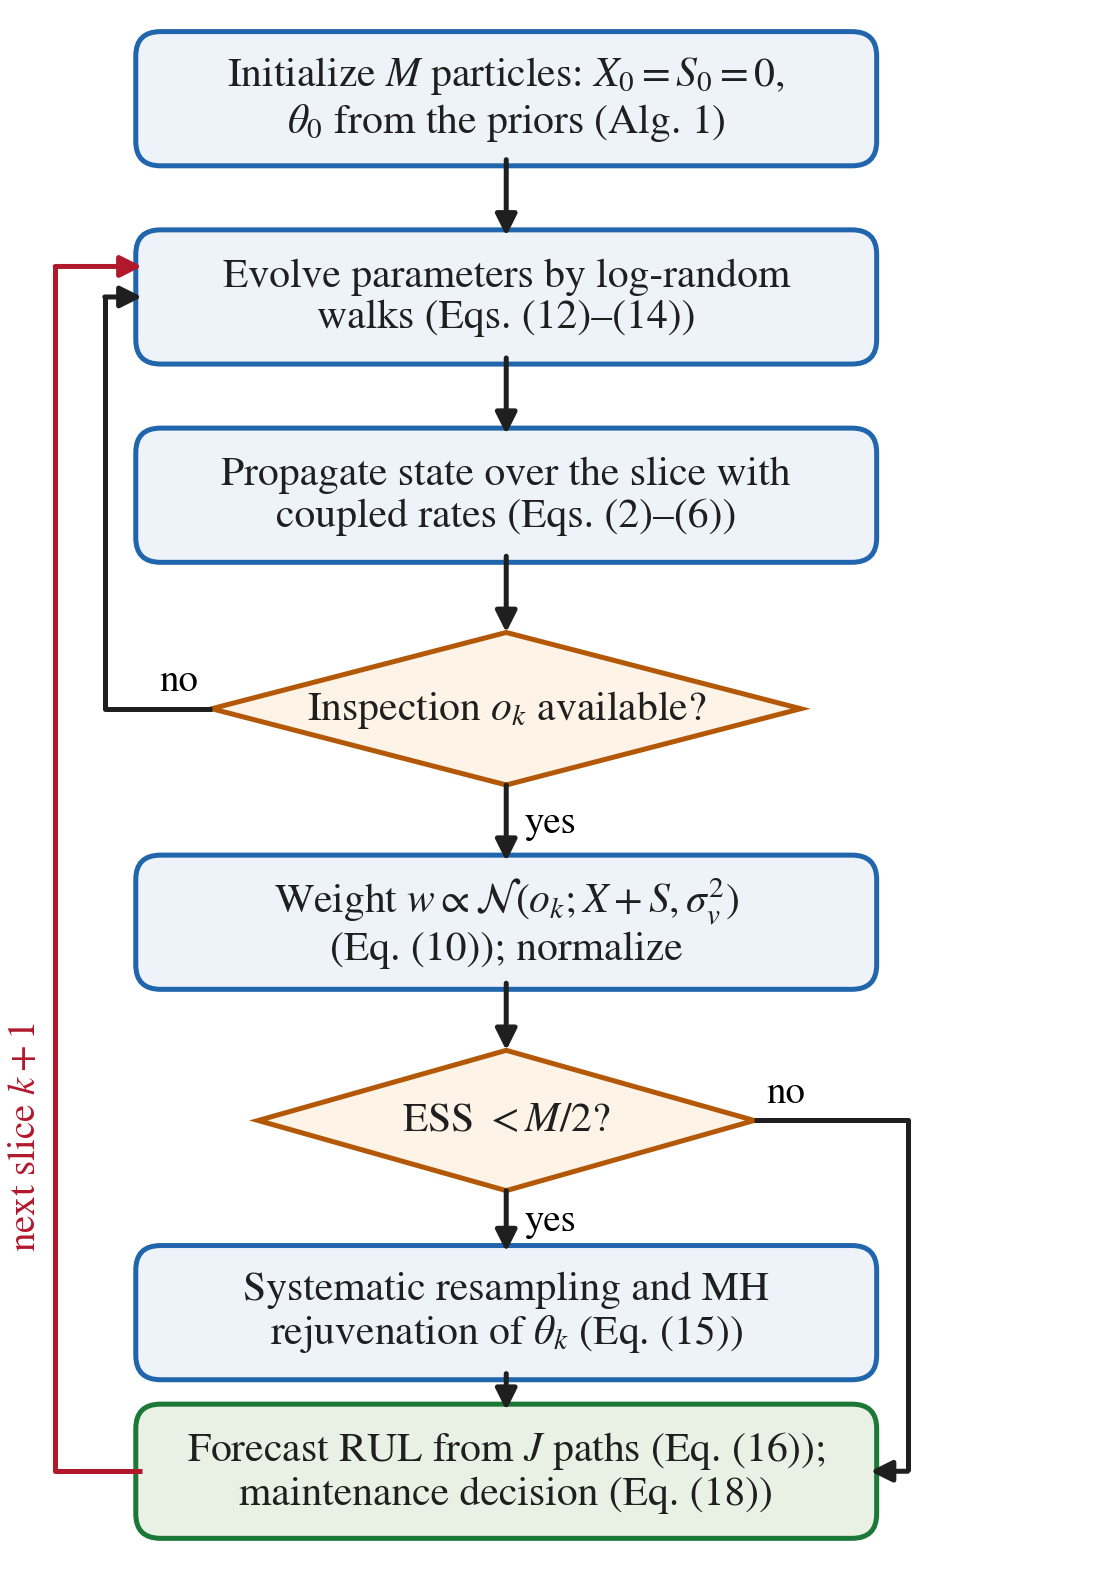
\includegraphics[width=0.85\linewidth]{figures/fig3_smcflow.png}
\caption{Particle-filter workflow corresponding to
Algorithm~\ref{alg:smc}: parameter evolution, state propagation,
observation weighting, resampling, and MCMC rejuvenation, followed by
the RUL forecast and maintenance decision of Section~\ref{sec:cost}.}
\label{fig:flow}
\end{figure}


% ------------------------------------------------------------
% III-C
% ------------------------------------------------------------

\subsection{Posterior RUL Prediction and Maintenance Decision Model}
\label{sec:cost}

The posterior distribution obtained after assimilating the available
inspection observations provides a probabilistic representation of
the current degradation state and adaptive model parameters. To
translate this posterior information into a prognostic quantity, the
posterior particle population is propagated forward without further
measurements.

Given the filtering distribution at inspection time
$t_{\mathrm{curr}}$, $J=10{,}000$ future degradation trajectories are
generated, each starting from a particle drawn from the filtering
distribution; along each trajectory the baseline parameters continue
their random walk. For trajectory $j$, the predicted failure time is

\begin{equation}
t_{\mathrm{fail}}^{(j)}
=
\inf
\left\{
\tau>t_{\mathrm{curr}}:
P_{\mathrm{burst}}(Z(\tau))
\le
P_{\mathrm{op}}
\right\},
\label{eq:rul}
\end{equation}

with

\[
\mathrm{RUL}^{(j)}
=
t_{\mathrm{fail}}^{(j)}
-
t_{\mathrm{curr}}.
\]

The resulting ensemble of failure times defines the predictive RUL
distribution. The 10th percentile of this distribution is used as a
conservative RUL quantity for maintenance decision support.

The maintenance policy is parameterized by the inspection interval $I$
and the preventive-maintenance threshold $\gamma$. Inspections take
place at $t=I,2I,\dots$ within the planning horizon $T$. At each
inspection the filter assimilates the measurement and the RUL forecast
is recomputed; preventive replacement is ordered when the 10th
percentile of the forecast RUL is at most $\gamma$, that is, when
$\Pr(\mathrm{RUL}\le\gamma)\ge0.1$. A failure between inspections
(Eq.~\eqref{eq:burstfail}) triggers corrective replacement at the
failure time. Either replacement resets the damage state to zero while
the parameter posterior is retained, because the environment is
unchanged, and the inspection schedule continues. The expected
discounted lifecycle cost is estimated by simulating this closed loop
on $N_p$ pipelines:

\begin{equation}
\resizebox{0.90\linewidth}{!}{$\displaystyle
\mathbb{E}[C_{\mathrm{total}}(I,\gamma)]
\approx
\frac{1}{N_p}
\sum_{n=1}^{N_p}
\Bigl[
\sum_{t\in\mathcal{T}_{\mathrm{ins}}}\frac{C_{\mathrm{ins}}}{(1+r)^{t}}
+
\sum_{t\in\mathcal{T}^{(n)}_{\mathrm{prev}}}\frac{C_{\mathrm{prev}}}{(1+r)^{t}}
+
\sum_{t\in\mathcal{T}^{(n)}_{\mathrm{fail}}}\frac{C_{\mathrm{fail}}+C_{\mathrm{env}}}{(1+r)^{t}}
\Bigr]$}
\label{eq:cost}
\end{equation}

where $\mathcal{T}_{\mathrm{ins}}$ is the set of inspection times,
$\mathcal{T}^{(n)}_{\mathrm{prev}}$ and $\mathcal{T}^{(n)}_{\mathrm{fail}}$
are the times of the preventive and corrective replacements of pipeline
$n$, $C_{\mathrm{ins}}$, $C_{\mathrm{prev}}$, and $C_{\mathrm{fail}}$ are
the inspection, preventive-repair, and corrective-repair costs,
$C_{\mathrm{env}}$ is the environmental penalty incurred at failure, and
$r$ is the discount rate. Because the costs are those incurred by the
simulated pipelines, a model is not rewarded for forecasting longer
lives.

The optimal maintenance policy is defined as

\begin{equation}
(I^*,\gamma^*)
=
\arg\min_{I,\gamma}
\mathbb{E}
[C_{\mathrm{total}}(I,\gamma)].
\label{eq:opt}
\end{equation}

The search grid, planning horizon, and economic parameters are given in
Section~\ref{sec:metrics}.

% ============================================================
% END OF SECTION III
% Section IV should begin immediately after this block.
% ============================================================
%-----------------------------
% ============================================================
% IV. EXPERIMENTAL SETUP AND EVALUATION PROTOCOL
% ============================================================

\section{Experimental Setup and Evaluation Protocol}
\label{sec:evalsetup}

The API-DBN is evaluated using two complementary sources of
information. Historical BSEE/NETL Gulf of Mexico pipeline and incident
records are used to check the parameter assumptions, whereas
controlled simulations provide
trajectories with known failure times for quantitative assessment of
RUL prediction.
This distinction is necessary because the historical records do not
contain complete longitudinal inspection histories or true RUL labels
for all pipeline segments. The experimental protocol therefore labels
each parameter as an assumption or a case value, states which of them
were checked against the records, and evaluates predictive performance
only where ground truth is available.


% ------------------------------------------------------------
% IV-A
% ------------------------------------------------------------

\subsection{Historical Records}
\label{sec:data}

Historical information is taken from the U.S.\ Offshore Pipeline and
Reported Incident Datasets, which NETL compiled from BSEE, PHMSA, and
other public sources \cite{romeo2024,pfander2024}. Four files of the
Energy Data eXchange submission were downloaded on 29~September~2026:
the incident table \texttt{pipeline\_incidents.csv} (uploaded
11~January~2024; 943 incident reports with 85 fields), the
location table \texttt{pipeline\_locations.csv} (uploaded
17~January~2024; 89{,}986 points along 14{,}241 BSEE pipeline
segments, with 495 columns), and their field dictionaries
\texttt{pipeline\_incidents\_data\_dictionary.csv} and
\texttt{pipeline\_location\_data\_dictionary.csv}.
Table~\ref{tab:bsee} summarizes the records.

The records are processed as follows. The year of an incident is taken
from its reported local date. Diameter, wall thickness, and SMYS are
treated as missing when empty or non-positive, wall thicknesses above
2~in and SMYS values above 120~ksi are treated as invalid, and SMYS
values below 1{,}000 are read as ksi. Missing values are not imputed:
each statistic uses only the records in which the field is reported,
and Table~\ref{tab:bsee} gives the number of such records. Segments are
identified by their BSEE segment number; diameter, length, status, and
dates are identical on all points of a segment. Proposed and cancelled
segments are excluded. The exposure of a segment runs from its
installation date, or 1~January~1986 if later, to its abandonment date,
or 31~December~2021 if it is later or absent; segments without an
installation date, and segments without an abandonment date that are
neither active nor out of service, are left out of the exposure. Costs
are the reported totals in 2021 U.S.\ dollars. The records are not
partitioned into training, validation, and test sets, because no model
parameter is fitted to them and no held-out evaluation is reported
(Section~\ref{sec:case_results}).



\begin{table}[t]
\centering
\caption{Summary of the BSEE/NETL Records}
\label{tab:bsee}
\footnotesize
\begin{tabular}{lr}
\toprule
Quantity & Value \\
\midrule
Incident reports (PHMSA / BSEE) & 943 (889 / 54) \\
Years of the incidents & 1986--2021 \\
Reports with lease block (distinct blocks) & 881 (487) \\
Internal / external corrosion flagged & 355 / 94 \\
Outside-force damage flagged & 158 \\
Diameter / wall / SMYS reported & 779 / 734 / 705 \\
Positive reported cost & 831 \\
Location points & 89{,}986 \\
Installed segments (with size code) & 14{,}202 (13{,}792) \\
Segments with known exposure & 11{,}236 \\
Segment-years, 1986--2021 & 185{,}497 \\
\bottomrule
\end{tabular}
\end{table}

The records serve three checks of the simulation assumptions, not
parameter estimation. First, the case segment of
Table~\ref{tab:simparams} (outside diameter 0.61~m, or 24~in; wall
19.1~mm, or 0.75~in; API~5L X52) is a large trunkline rather than a
typical segment: 1.5\% of the installed segments with a size code
are 24~in or larger (median 6~in), and the median wall thickness
of the pipes involved in incidents is 0.41~in (10.4~mm). Its
grade is the most frequently reported one (X52 in 250 of the 705
reports that give SMYS). Second, the 943 reports correspond to
0.0051 incidents per segment-year of exposure. This is an upper bound,
because segments with unknown dates are left out of the exposure, and
it is far below the modelled shock rate $\lambda=0.8$~yr$^{-1}$: shocks
in the present model include minor impacts that do not produce
reportable incidents, so the incident frequency is not an estimate of
$\lambda$, which remains an assumption. Third, the failure cost
$C_{\mathrm{fail}}=\$5$M of Table~\ref{tab:costparams} exceeds the
reported cost of 91.7\% of the 831 incidents with a positive cost
(median \$0.33M, mean \$2.84M), so it represents a severe failure
rather than a typical incident.

Table~\ref{tab:simparams} records the value and provenance of each
quantity used in the controlled simulations.

\begin{table}[t]
\centering
\caption{Model Parameters Used in Simulation, with Source}
\label{tab:simparams}
\begin{tabular}{p{0.9cm}p{1.2cm}p{2.5cm}p{2.6cm}}
\toprule
Parameter & Value & Description & Source \\
\midrule
$\mu_{\mathrm{base}}$ & 0.44 mm/yr & Baseline corrosion drift & Assumption \\
$\sigma_B$ & 0.20 mm/yr$^{1/2}$ & Diffusion coefficient & Assumption \\
$\lambda$ & 0.8 yr$^{-1}$ & Baseline shock rate & Assumption (Sec.~\ref{sec:data}) \\
$\mu_{y_0}$ & 0.32 mm & Mean shock magnitude $Y$ & Assumption \\
$\sigma_{y_0}$ & 0.15 mm & Std.\ dev.\ of $Y$ & Assumption \\
$W_0$ & 1.0 mm & Sigmoid midpoint & Assumption; sensitivity in Sec.~\ref{sec:data} \\
$\alpha$ & 2.0 & Acceleration factor & Assumption; sensitivity in Sec.~\ref{sec:data} \\
$r_s$ & 0.5 mm$^{-1}$ & Sigmoid steepness & Assumption; sensitivity in Sec.~\ref{sec:data} \\
$M$ & 1{,}000 & Number of particles & Convergence check, Sec.~\ref{sec:data} \\
$K$ & 200 & Time steps ($\Delta t=0.1$~yr, 20-yr horizon) & Assumption \\
$J$ & 10{,}000 & RUL forecast trajectories & Convergence check, Sec.~\ref{sec:data} \\
\midrule
$\kappa$ & 0.30 & Shock-to-equivalent-damage scaling & Assumption \\
$\eta$ & 0.50 & Shock-damage exponent & Assumption \\
$\gamma_1$ & 0.05 mm$^{-1}$ & Corrosion effect on shock intensity & Assumption \\
$\sigma_\mu$ & 0.05 & Drift random-walk SD (log scale, per year) & Assumption (parameter tracking) \\
$\sigma_\lambda$ & 0.05 & Shock-rate random-walk SD (log scale, per year) & Assumption (parameter tracking) \\
$\sigma_\sigma$ & 0.05 & Diffusion random-walk SD (log scale, per year) & Assumption (parameter tracking) \\
$\sigma_v$ & 0.10 mm & Inspection error SD & Modelling assumption (idealized inspection accuracy) \\
$D$ & 0.61 m & Pipeline diameter & Case value (24-in trunkline; Sec.~\ref{sec:data}) \\
$t_{\mathrm{nom}}$ & 19.1 mm & Nominal wall thickness & Case value \\
$L$ & 0.50 m & Defect length & Case value \\
SMYS & 358 MPa & Material yield strength & Case value (API 5L X52; Sec.~\ref{sec:data}) \\
$P_{\mathrm{op}}$ & 10 MPa & Operating pressure & Case value \\
\bottomrule
\end{tabular}
\end{table}

\textit{Sensitivity and convergence.}
The sensitivity of the simulated lifetime to the coupling parameters
was examined by varying one parameter at a time, with the others at
their Table~\ref{tab:simparams} values (10{,}000 trajectories each).
The median time to failure changes little for $W_0$ between 0.25 and
2~mm (12.3--12.9~yr) and for $r_s$ between 0.25 and 5~mm$^{-1}$
(12.2--13.0~yr), but strongly with the acceleration factor: $\alpha=1$,
2, and 3 give 19.9, 12.5, and 9.2~yr. The value of $\alpha$ is
therefore the dominant coupling assumption. Filter accuracy was
insensitive to the particle number: on the same 80 pipelines, the RUL
MAE of API-DBN varied between 1.01 and 1.04~yr for
$M\in\{250,500,1000,2000\}$, so $M=1{,}000$ is conservative. With
$J=10{,}000$ forecast trajectories, the Monte Carlo standard deviation
of the 2.5th and 97.5th RUL percentiles was 0.02 and 0.06~yr (0.07 and
0.15~yr with $J=1{,}000$).


% ------------------------------------------------------------
% IV-B
% ------------------------------------------------------------

\subsection{Controlled Simulation Design, Baselines, and Ablations}
\label{sec:simsetup}

Quantitative RUL evaluation is performed using controlled degradation
simulations because the corresponding failure times are known exactly
within the simulated environment. Each simulated pipeline receives its
own baseline parameters $(\mu^{(0)},\lambda^{(0)},\sigma_B)$, equal to
the Table~\ref{tab:simparams} values multiplied by independent
$\exp(\varepsilon)$ with $\varepsilon\sim\mathcal{N}(0,0.25^2)$, which
then drift annually by the log-random walks of
Eqs.~\eqref{eq:muwalk}--\eqref{eq:sigmaBwalk} with the standard
deviations in Table~\ref{tab:simparams}. Degradation follows the
corrosion, shock, coupling, and structural-failure formulations of
Section~\ref{sec:physics}, simulated with $\Delta t=0.1$~yr ($K=200$
steps over a 20-yr monitoring window) until $Z\ge d_{\mathrm{crit}}$.
Each pipeline is inspected annually from $t=1$~yr; every inspection
before failure yields an observation through Eq.~\eqref{eq:obs} with
independent Gaussian noise of standard deviation $\sigma_v$, and no
observations are missing. Performance statistics are evaluated over 30
independent runs with random seeds 0--29, each containing 333 pipelines
(9{,}990 in total). A second design, in which every pipeline has
exactly the Table~\ref{tab:simparams} parameters, is reported for
comparison.

Because the controlled trajectories are generated from the same model
family used for API-DBN inference, the experiment evaluates performance
under model-consistent conditions; it does not establish robustness to
model-form misspecification.

Five model configurations are evaluated under the same controlled
simulation conditions:

\begin{enumerate}
    \item \textit{Fixed Wiener}: a linear Wiener process on the total
    damage $Z$ whose drift and diffusion are fitted by moments to the
    inspection increments of 2{,}000 separately simulated training
    pipelines; the latest observation is taken as the current state,
    and the RUL follows the inverse-Gaussian first-passage distribution;

    \item \textit{Static DBN}: the proposed model and particle filter
    with the parameters fixed at the Table~\ref{tab:simparams} values,
    that is, offline calibration without parameter updating, following
    the static formulation of \cite{liu2023};

    \item \textit{PF without MCMC}: the adaptive particle filter without
    the MCMC rejuvenation step;

    \item \textit{No coupling}: the adaptive model with MCMC
    rejuvenation in which the coupling of
    Eqs.~\eqref{eq:mueff}--\eqref{eq:lambdaeff} is disabled
    ($\alpha=1$, $\gamma_1=0$); and

    \item \textit{API-DBN}: the complete proposed framework with
    sequential state and parameter updating, MCMC rejuvenation, and
    state-dependent corrosion--shock coupling.
\end{enumerate}

Two reference configurations complete the analysis: the adaptive model
without both coupling and MCMC, which makes the ablation a full
$2\times2$ factorial design, and an oracle that knows each pipeline's
true parameters and therefore bounds the achievable error.

The same random seeds and corresponding trajectory sets are used across
the compared models. This matched design reduces variation associated
with different simulated realizations and supports paired statistical
comparison of the resulting performance metrics.

The four adaptive configurations form a $2\times2$ factorial design in
coupling and MCMC rejuvenation, so the effect of each component can be
isolated; the static DBN and fixed Wiener models differ from them in
more than one respect and serve as external baselines.


% ------------------------------------------------------------
% IV-C
% ------------------------------------------------------------

\subsection{Evaluation Metrics, Statistical Tests, and Computational Protocol}
\label{sec:metrics}

RUL prediction is evaluated using Mean Absolute Error (MAE), Root Mean
Squared Error (RMSE), Continuous Ranked Probability Score (CRPS),
Brier Score, and 95\% Prediction Interval Coverage Probability (PICP).
MAE and RMSE quantify point-prediction error, whereas CRPS evaluates
the complete predictive RUL distribution. The Brier Score evaluates
probabilistic failure prediction within the specified evaluation
window, and PICP measures empirical coverage of the nominal 95\%
RUL prediction interval.

For a predictive RUL distribution $F$ and realized outcome $y$, CRPS
is defined as

\begin{equation}
\mathrm{CRPS}(F,y)
=
\mathbb{E}_F|X-y|
-
\tfrac{1}{2}\mathbb{E}_F|X-X'|,
\label{eq:crps}
\end{equation}

where $X$ and $X'$ are independent draws from $F$.

The Brier Score is computed as

\begin{equation}
\mathrm{Brier}
=
\frac{1}{N}
\sum_{i=1}^{N}
\left(
p_i-\mathbb{1}[F_i]
\right)^2,
\label{eq:brier}
\end{equation}

where $p_i$ is the predicted probability of failure for test case
$i$, and $\mathbb{1}[F_i]$ indicates whether failure occurs within the
evaluation window.

Prediction-interval coverage is evaluated as

\begin{equation}
\mathrm{PICP}
=
\frac{1}{N}
\sum_{i=1}^{N}
\mathbb{1}
\left[
y_i\in CI_{95\%,i}
\right],
\label{eq:picp}
\end{equation}

where $CI_{95\%,i}$ is the nominal 95\% prediction interval for case
$i$. Here, $N$ denotes the number of test cases: one forecast at every
annual inspection before failure, giving $N=121{,}091$ forecasts per
model for the 9{,}990 test pipelines. The $J=10{,}000$ Monte Carlo
trajectories generated for an individual case are used to construct its
predictive RUL distribution and associated interval; they are not
treated as independent ground-truth observations. The point prediction
is the median of the predictive distribution, and the Brier score uses
the event that failure occurs within 2~yr of the inspection.

Statistical comparisons use the same 30 matched simulation runs
described in Section~\ref{sec:simsetup}. Because each model is applied
to the same random-seed realization, the per-run metric values form
paired samples. Differences between API-DBN and the comparison models
are therefore assessed using a paired $t$-test
\cite{montgomery2017}. For paired observations with mean difference
$\bar d$ and standard deviation of the differences $s_d$, the test
statistic is

\begin{equation}
t
=
\frac{\bar d}{s_d/\sqrt{n}},
\qquad
\mathrm{d.f.}=n-1=29,
\quad n=30.
\label{eq:ttest}
\end{equation}

The resulting statistical outcomes are reported with the corresponding
predictive-performance results in Section~\ref{sec:rulresults}, rather
than in the present experimental-protocol section.

Filtering-stage intervals are obtained from the $M=1{,}000$ particles.
The 95\% prediction interval of each RUL forecast is the central
interval between the 2.5th and 97.5th percentiles of the $J$ simulated
failure times \cite{efron1993}. Because every trajectory starts from a
particle drawn from the joint state--parameter posterior, the interval
reflects state, parameter, and future-process uncertainty.


% ------------------------------------------------------------
% Maintenance-policy evaluation protocol
% ------------------------------------------------------------

\textit{Maintenance-policy evaluation.}
The maintenance policy defined by Eq.~\eqref{eq:opt} is evaluated by
grid search over $I\in\{1.0,1.5,\dots,4.0\}$~yr and
$\gamma\in\{0.5,1.0,\dots,5.0\}$~yr over a planning horizon of
$T=20$~yr. For each candidate policy, Eq.~\eqref{eq:cost} is estimated
by running the closed loop of Section~\ref{sec:cost} on the same
$N_p=1{,}500$ simulated pipelines, generated as in
Section~\ref{sec:simsetup}; each pipeline's corrosion noise, shocks,
parameter drift, and inspection errors are drawn once and shared by all
policies and models (common random numbers). Each replacement decision
uses $2{,}000$ forecast trajectories, which estimate the 10\%
exceedance probability with a standard error of about 0.007.

The economic parameters used in the maintenance experiment are listed
in Table~\ref{tab:costparams}.

\begin{table}[t]
\centering
\caption{Cost Parameters, with Source}
\label{tab:costparams}
\begin{tabular}{p{1.2cm}p{2.0cm}p{0.9cm}p{2.2cm}}
\toprule
Parameter & Description & Value (\$k) & Source \\
\midrule
$C_{\mathrm{ins}}$ & AUV inspection & 50 & Assumption \\
$C_{\mathrm{prev}}$ & Preventive intervention & 200 & Assumption \\
$C_{\mathrm{fail}}$ & Corrective repair & 5{,}000 & Assumption; exceeds 92\% of reported incident costs (Sec.~\ref{sec:data}) \\
$C_{\mathrm{env}}$ & Environmental penalty & 10{,}000 & Assumption (regulatory-penalty proxy) \\
$r$ & Discount rate & 0.05 & Modelling assumption \\
\bottomrule
\end{tabular}
\end{table}




% ------------------------------------------------------------
% Computational protocol
% ------------------------------------------------------------

\textit{Computational protocol.}
The API-DBN experiments use $M=1{,}000$ particles and $K=200$ time
steps. Filtering scales as $O(MK)$, MCMC rejuvenation adds a
per-particle cost whenever the resampling criterion is satisfied, and
each RUL forecast scales as $O(JH)$ for a forecast horizon of $H$
steps. Runtimes were measured on an Apple M4 processor (10 cores,
16~GB RAM) running macOS, with Python~3.14, NumPy~2.5, and SciPy~1.18,
one pipeline per core, and averaged over the 30 runs. Observed
computational performance is reported in Section~\ref{sec:complexity}.

% ============================================================
% END OF SECTION IV
% ============================================================
% ============================================================
% V. RESULTS AND DISCUSSION
% ============================================================

\section{Results and Discussion}
\label{sec:results}

This section presents the predictive, maintenance-decision, and
computational results obtained using the experimental protocol defined
in Section~\ref{sec:evalsetup}, and then discusses the implications of
adaptive parameter updating, degradation--shock coupling, and posterior
uncertainty propagation, together with the limitations of the present
formulation.


% ------------------------------------------------------------
% V-A
% ------------------------------------------------------------

\subsection{RUL Prediction, Reliability, and Ablation Results}
\label{sec:rulresults}

Table~\ref{tab:rulresults} summarizes RUL prediction over the 30
matched runs (9{,}990 pipelines; 121{,}091 forecasts per model).
API-DBN attains an MAE of $1.12\pm0.04$~yr against $1.38\pm0.09$~yr
for the static DBN and $1.37\pm0.08$~yr for the fixed-parameter Wiener
model, a reduction of 18.6\%, and it reduces the CRPS by 28.7\% (0.80
versus 1.12~yr) and the RMSE by 16\%. The larger difference is in
calibration: the 95\% prediction intervals of API-DBN contain the true
RUL in 95.3\% of forecasts (Wilson 95\% interval 95.2--95.4\%), whereas
the static DBN, which cannot learn pipeline-specific rates, covers only
59.9\% with intervals less than half as wide (2.4 versus 6.1~yr). An
oracle that knows each pipeline's true parameters reaches an MAE of
0.70~yr, which bounds what any model can achieve; API-DBN closes 38\%
of the gap between the static DBN and this bound.

\begin{table}[t]
\centering
\caption{RUL Prediction Performance (Mean $\pm$ Std.\ over 30 Runs)}
\label{tab:rulresults}
\resizebox{\columnwidth}{!}{%
\begin{tabular}{lccccc}
\toprule
Model & MAE (yr) & RMSE (yr) & CRPS (yr) & Brier & PICP (\%) \\
\midrule
Fixed Wiener & $1.37\pm0.08$ & $1.96\pm0.14$ & $1.04\pm0.07$ & $0.031\pm0.002$ & 75.0 \\
Static DBN & $1.38\pm0.09$ & $2.05\pm0.16$ & $1.12\pm0.08$ & $0.032\pm0.002$ & 59.9 \\
PF w/o MCMC & $1.12\pm0.04$ & $1.73\pm0.08$ & $0.80\pm0.03$ & $0.022\pm0.001$ & 95.2 \\
No coupling & $2.29\pm0.07$ & $3.39\pm0.10$ & $1.67\pm0.05$ & $0.027\pm0.001$ & 77.5 \\
\textbf{API-DBN} & $\mathbf{1.12\pm0.04}$ & $\mathbf{1.72\pm0.08}$ & $\mathbf{0.80\pm0.03}$ & $\mathbf{0.021\pm0.001}$ & \textbf{95.3} \\
\midrule
No coupling, w/o MCMC & $2.29\pm0.06$ & $3.38\pm0.10$ & $1.67\pm0.05$ & $0.027\pm0.002$ & 77.3 \\
Oracle (true parameters) & $0.70\pm0.03$ & $1.04\pm0.06$ & $0.50\pm0.02$ & $0.018\pm0.001$ & 95.4 \\
\bottomrule
\end{tabular}}
\end{table}

Paired $t$-tests over the 30 matched runs confirm that API-DBN improves
on the static DBN for every metric: MAE $t_{29}=17.7$, RMSE
$t_{29}=13.8$, CRPS $t_{29}=23.6$, and Brier score $t_{29}=29.7$ (all
$p<10^{-13}$). The Brier scores are small for all models because
failure within 2~yr of an inspection is a minority event among the
pooled forecasts.

\textit{Ablation results.}
Table~\ref{tab:ablation} isolates the two components within the
adaptive model. Removing the corrosion--shock coupling doubles the MAE,
from 1.12 to 2.29~yr: the adaptive drift then has to absorb an
acceleration it cannot anticipate, and the RUL is overestimated by
2.1~yr on average. MCMC rejuvenation, in contrast, has no measurable
effect with or without coupling (PF without MCMC versus API-DBN:
$t_{29}=-0.05$, $p=0.96$). With the state held fixed, the move of
Eq.~\eqref{eq:mh} can only refresh $\theta_k$ within the random-walk
spread around $\theta_{k-1}$, which the random walk of
Eqs.~\eqref{eq:muwalk}--\eqref{eq:sigmaBwalk} already provides.

\begin{table}[t]
\centering
\caption{Factorial Ablation of the Adaptive Model (MAE, yr)}
\label{tab:ablation}
\begin{tabular}{lcc}
\toprule
 & Coupling off & Coupling on \\
\midrule
MCMC off & 2.29 & 1.12 \\
MCMC on & 2.29 & 1.12 \\
\bottomrule
\end{tabular}
\end{table}

\textit{Identical parameters.}
When every pipeline has exactly the Table~\ref{tab:simparams}
parameters (3{,}000 pipelines, 36{,}090 forecasts per model), the static
DBN coincides with the oracle (MAE 0.48~yr) and outperforms API-DBN
(0.93~yr; $t_{29}=-56.0$), because the adaptive model must learn
parameters that are already known. Sequential parameter updating
therefore pays off when parameters differ between assets or drift over
time, which is the situation it is designed for.

\textit{Degradation trajectories.}
Figure~\ref{fig:trajectories} shows equivalent-damage trajectories
simulated with the Table~\ref{tab:simparams} parameters for shock rates
$\lambda=0.3$, $0.8$, and $1.5~\mathrm{yr}^{-1}$. Mean damage at 20~yr
is 18.0, 20.6, and 24.4~mm, and the median time to reach the
Eq.~\eqref{eq:burstfail} failure depth of 12.1~mm is 14.0, 12.5, and
11.0~yr, respectively. Because the sigmoid factor of
Eq.~\eqref{eq:mueff} is at least 1.38, the corrosion drift never falls
below 0.61~mm/yr, so every simulated pipeline fails within 16~yr even
at the lowest shock rate.

\begin{figure}[t]
\centering
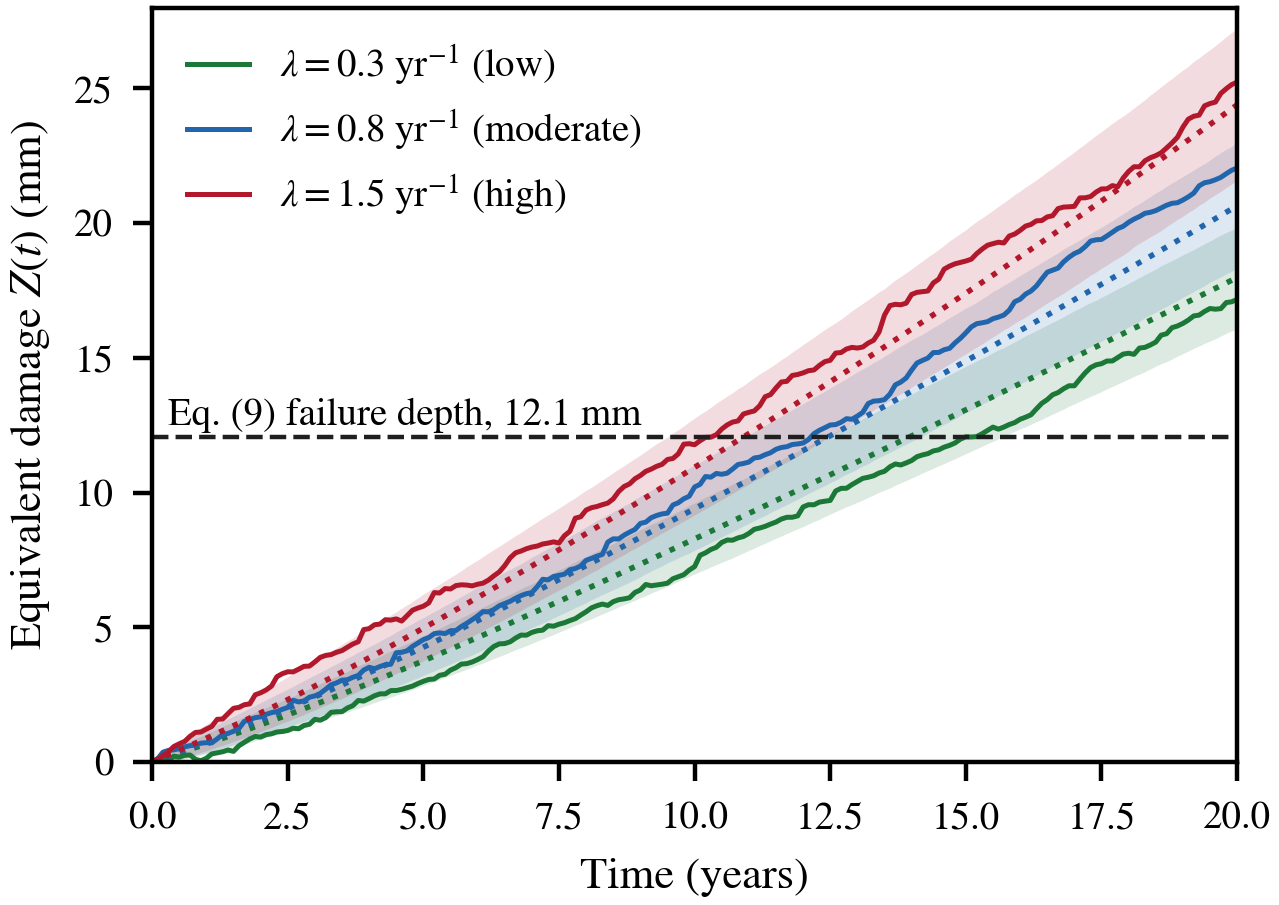
\includegraphics[width=\linewidth]{figures/fig4_trajectories.png}
\caption{Equivalent damage simulated with the Table~\ref{tab:simparams}
parameters for shock rates $\lambda=0.3$, $0.8$, and $1.5$~yr$^{-1}$:
one path (solid), the mean (dotted), and the 5--95\% band of 10{,}000
paths (shaded). The dashed line is the depth at which
Eq.~\eqref{eq:burstfail} holds (12.1~mm).}
\label{fig:trajectories}
\end{figure}

\textit{Reliability.}
Figure~\ref{fig:reliability}(a) compares the true reliability of the
simulated population with the reliability each model implies before any
inspection, and Fig.~\ref{fig:reliability}(b) shows the conditional
reliability of one pipeline after six annual inspections. With the
Table~\ref{tab:simparams} parameters the true reliability stays above
0.99 until 10~yr and falls below 0.01 by 15~yr (median life 12.5~yr).
After six inspections, the API-DBN forecast for the example pipeline
lies close to the oracle, whereas the static DBN, which applies the
population parameters, predicts a later failure. A reliability curve is
a forecast; its quality is judged by the calibration metrics of
Section~\ref{sec:metrics}, not by its height.

\begin{figure}[t]
\centering
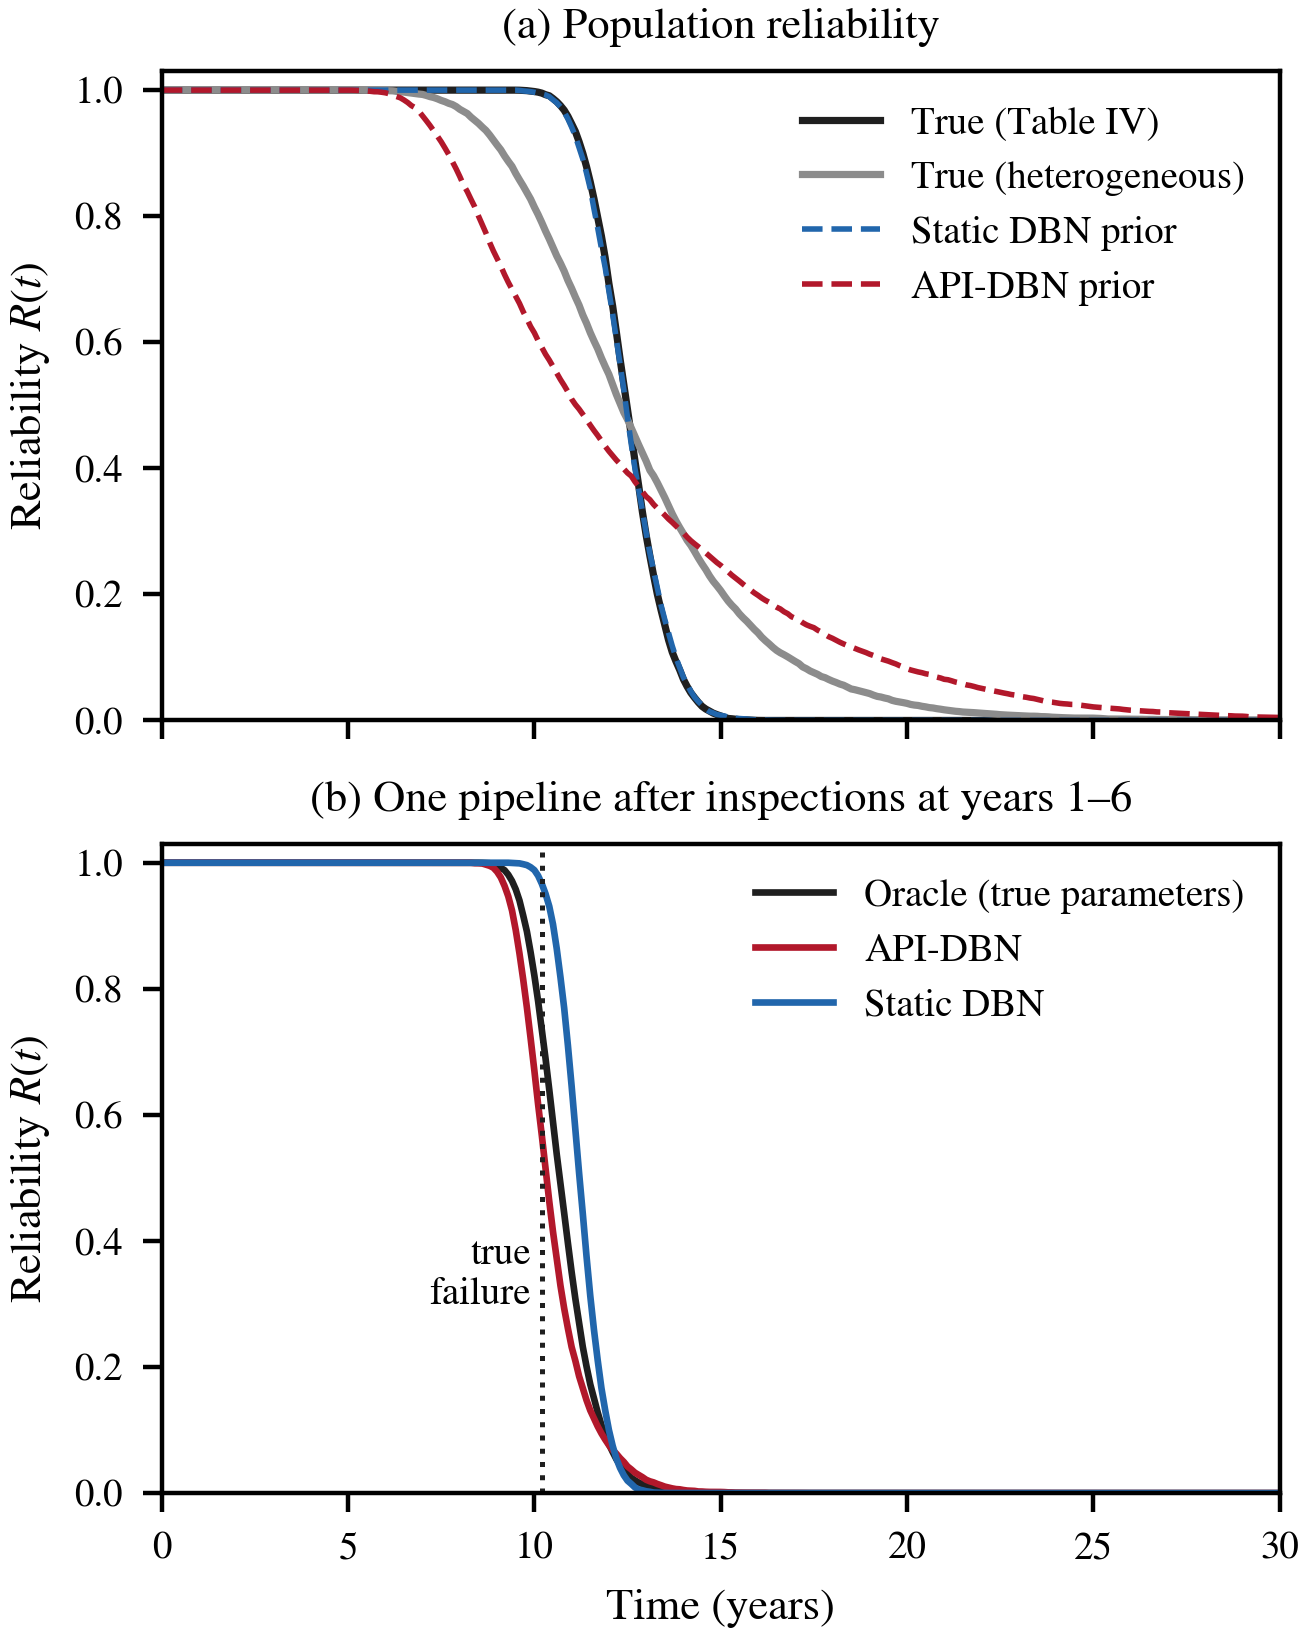
\includegraphics[width=\linewidth]{figures/fig5_reliability.png}
\caption{(a) Reliability of the simulated population with the
Table~\ref{tab:simparams} parameters and with pipeline-to-pipeline
variation, and the reliability implied by the static DBN and by the
API-DBN prior before any inspection. (b) Conditional reliability of one
pipeline with heterogeneous parameters after inspections at years 1--6;
the dotted line marks its true failure time.}
\label{fig:reliability}
\end{figure}


% ------------------------------------------------------------
% V-B
% ------------------------------------------------------------

\subsection{Maintenance Optimization Results}
\label{sec:costresults}

Each model operated the same 1{,}500 simulated pipelines over the
20-yr horizon with the closed loop of Section~\ref{sec:cost}.
Figure~\ref{fig:cost} shows the expected discounted lifecycle cost over
the policy grid, and Table~\ref{tab:maint} lists the cost-minimizing
policies. With the static DBN, the expected cost is minimized at
$I=2.5$~yr and $\gamma=4.5$~yr
(\$425k); with API-DBN it is minimized at
$I=4.0$~yr and $\gamma=5.0$~yr
(\$353k), which is 17\% lower and 3\% above the cost of a policy based
on the true parameters (\$342k). The API-DBN and oracle minima lie at the longest inspection interval
considered ($I=4$~yr), and the API-DBN minimum also lies at the largest
threshold ($\gamma=5$~yr), so policies beyond the searched domain could
lower these costs further; the static-DBN minimum lies inside the
domain. Policies with $\gamma<I$ leave
degraded pipelines unprotected until the next inspection: at $I=2$~yr
and $\gamma=1.5$~yr, 13--21\% of pipelines fail and
the expected cost rises to \$1.4--2.3M. The change in
prognostic information produced by sequential state and parameter
updating therefore propagates to the maintenance-decision layer and
lowers the cost of the policy it selects.

\begin{table}[t]
\centering
\caption{Cost-Minimizing Maintenance Policies (1{,}500 Pipelines, 20-yr Horizon)}
\label{tab:maint}
\resizebox{\columnwidth}{!}{%
\begin{tabular}{lcccc}
\toprule
Decision model & $I^*$ (yr) & $\gamma^*$ (yr) & Cost (\$k) & Pipelines failing (\%) \\
\midrule
Static DBN & 2.5 & 4.5 & $425.0\pm4.2$ & 0.07 \\
API-DBN & 4.0 & 5.0 & $353.5\pm4.8$ & 0.07 \\
Oracle (true parameters) & 4.0 & 4.5 & $342.1\pm11.1$ & 0.27 \\
\bottomrule
\end{tabular}}
\end{table}

\begin{figure*}[t]
\centering
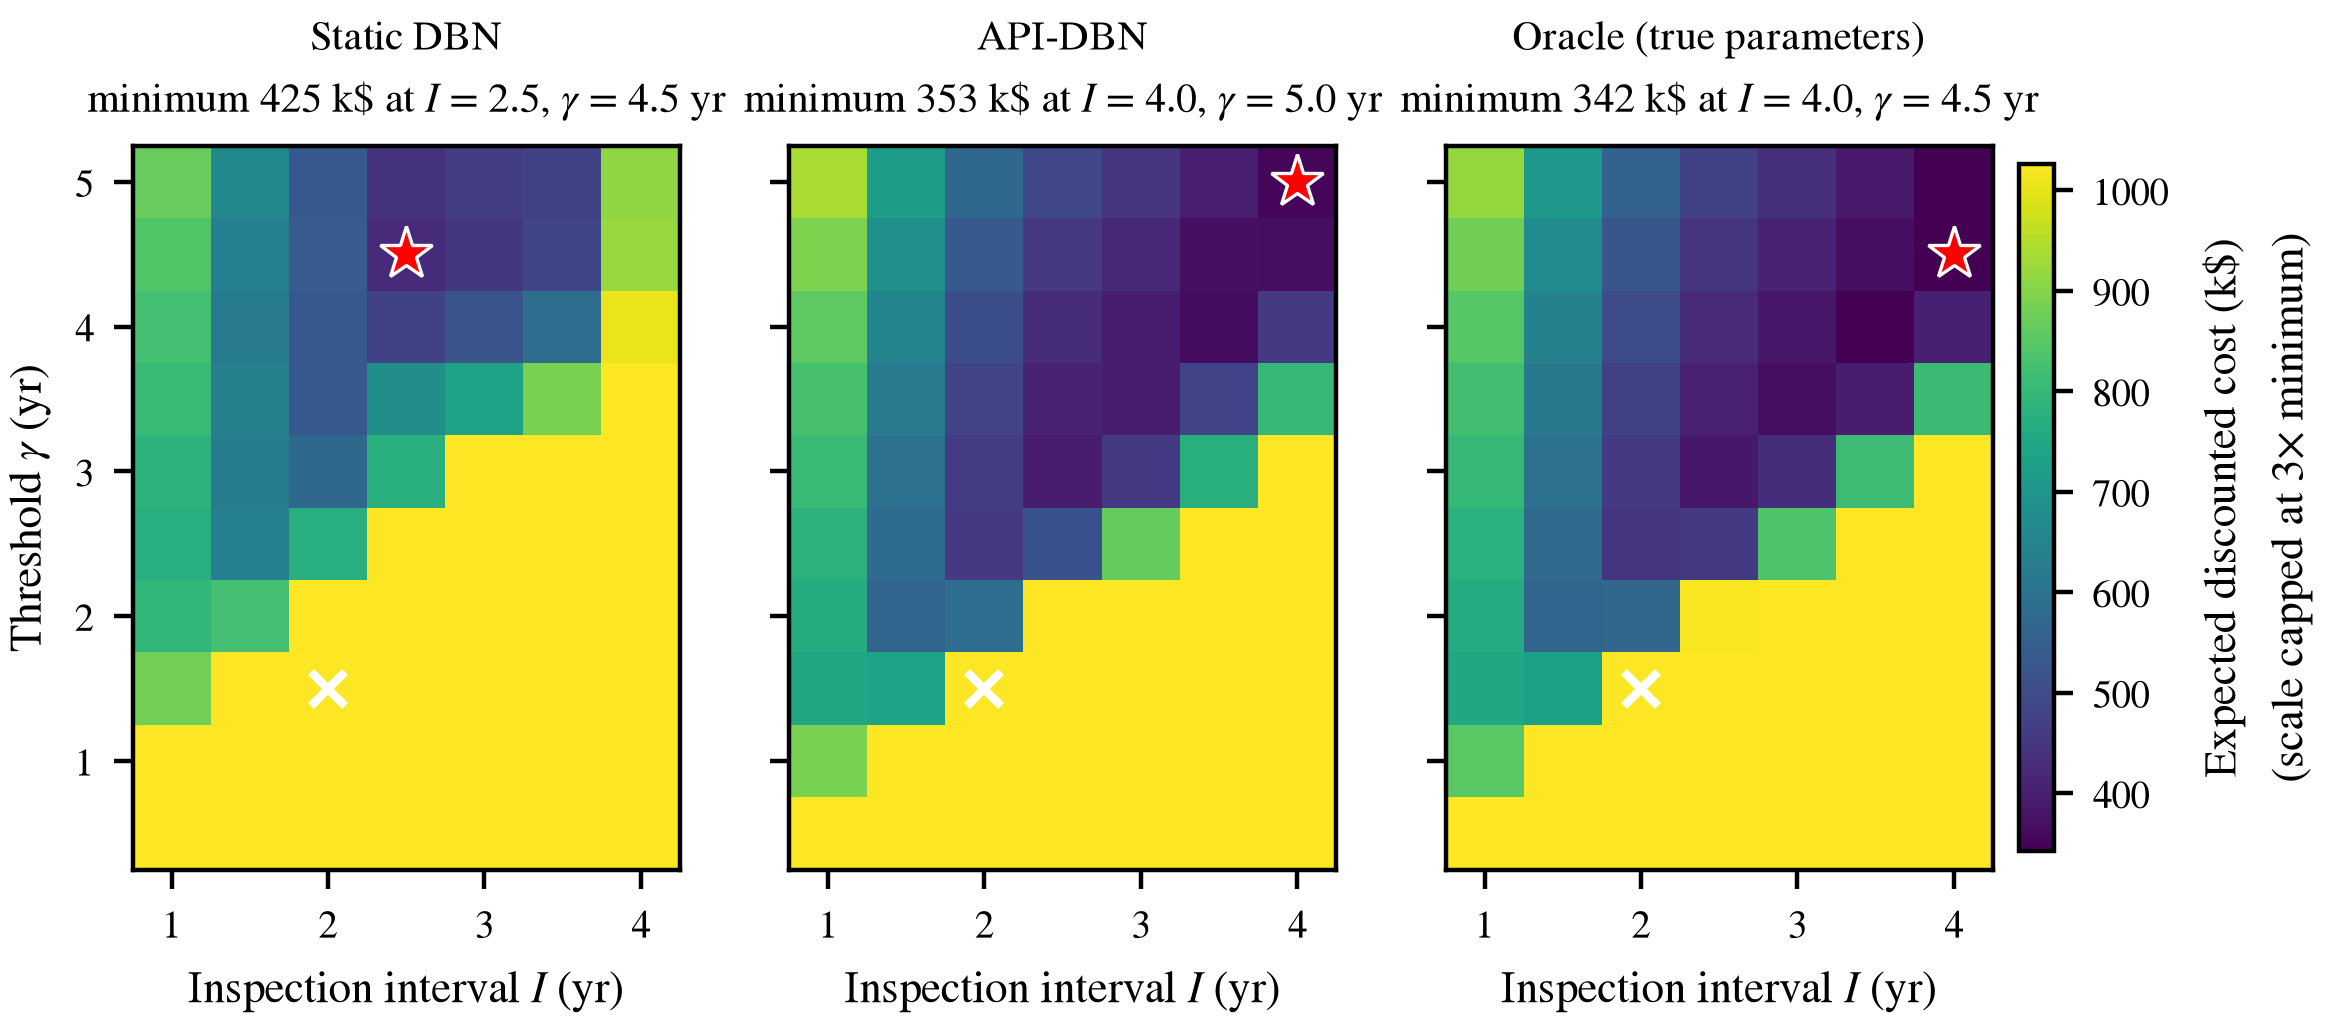
\includegraphics[width=\textwidth]{figures/fig6_cost.png}
\caption{Expected discounted lifecycle cost (k\$) when each model makes the
inspection and replacement decisions for the same 1{,}500 simulated
pipelines, over the inspection interval $I$ and the threshold $\gamma$
on the 10th-percentile RUL. Stars mark the minima; crosses mark the
policy $I=2$~yr, $\gamma=1.5$~yr. Policies with $\gamma<I$ allow failures
between inspections.}
\label{fig:cost}
\end{figure*}


% ------------------------------------------------------------
% V-C
% ------------------------------------------------------------

\subsection{Use of Historical Records}
\label{sec:case_results}

The BSEE/NETL records are used only for the checks of
Section~\ref{sec:data}. They contain neither longitudinal inspection
histories nor failure-time labels, so they cannot be used to validate
RUL prediction directly. A quantitative evaluation of incident risk,
for example the discrimination and calibration of predicted
segment-level failure probabilities against incidents reported after a
calibration period, is a natural next step. It is not reported here,
the records are not partitioned for it, and no claim of historical
validation is made.




% ------------------------------------------------------------
% V-D
% ------------------------------------------------------------

\subsection{Computational Performance}
\label{sec:complexity}

With $M=1{,}000$ particles, filtering over the $K=200$ time steps takes
0.05--0.07~s per pipeline for API-DBN (0.04~s without MCMC
rejuvenation), and a complete evaluation including about 12 RUL
forecasts with $J=10{,}000$ trajectories takes 1.1--1.3~s, measured on
the platform described in Section~\ref{sec:metrics}. The forecasts,
not the $O(MK)$ filter, therefore dominate the runtime. Because
pipelines are independent, the computation parallelizes across cores:
all seven configurations were evaluated for the 9{,}990 pipelines in
about 2~h on the 10-core processor.

The measured runtime indicates that the proposed inference procedure is
computationally tractable at the scale evaluated in this study. The
result should nevertheless be interpreted as an implementation
benchmark under the reported experimental configuration rather than as
evidence of fleet-scale or real-time deployment.


% ------------------------------------------------------------
% V-E
% ------------------------------------------------------------

\subsection{Scientific Discussion and Limitations}
\label{sec:discussion}

The controlled experiments indicate that the advantage of the API-DBN
arises from updating the baseline parameters as inspection evidence
accumulates, and that it appears when parameters differ between
pipelines or drift over time: with pipeline-specific, drifting
parameters, API-DBN reduces the MAE by 19\% and restores nominal
interval coverage, whereas with identical, known parameters the static
DBN performs better. The posterior error in the corrosion drift of
API-DBN falls from about 21\% after the first inspection to about 12\%
after ten and then stabilizes, because the random walk of
Eqs.~\eqref{eq:muwalk}--\eqref{eq:sigmaBwalk} gradually discounts old
evidence; this limits how closely the adaptive model can approach the
oracle.

The ablation results support retaining an explicit dependence between
progressive corrosion and discrete shock damage: without it, the
adaptive model is the least accurate configuration, because it
overestimates the remaining life of pipelines whose corrosion
accelerates. The MCMC rejuvenation step, as formulated here, does not
improve accuracy; a move that targets the parameter posterior given the
whole inspection history \cite{gilks2001} may be needed for
rejuvenation to contribute.

A second implication concerns uncertainty propagation. The API-DBN
does not terminate at a point estimate of the current degradation
state. The posterior state and parameter population is propagated to
a distribution of future failure times, allowing maintenance decisions
to depend on predictive uncertainty rather than on a single
deterministic RUL estimate. The maintenance results show that this
difference in prognostic information can propagate to the
decision layer: the API-DBN-based policy produces a lower expected
lifecycle cost than the policy obtained from the static-DBN RUL
distribution under the same cost model. This interpretation is
conditional on the economic assumptions in
Table~\ref{tab:costparams}; the reported optimum should not be assumed
to transfer directly to assets with different intervention costs,
failure consequences, or operational constraints.

The results should also be interpreted in view of the controlled
simulation design. The synthetic trajectories are generated from the
same general degradation-process family used by the inference model.
They therefore provide a controlled assessment under model-consistent
conditions but do not establish robustness to degradation-model
misspecification. Evaluation under alternative corrosion laws, shock
distributions, or coupling relationships would be required to
quantify sensitivity to structural model error.

Several modeling assumptions further limit the present formulation.
The Wiener process provides a tractable representation of stochastic
corrosion evolution but permits non-monotonic latent increments,
whereas physical wall loss is intrinsically cumulative. A Gamma
process or another monotonic degradation model may therefore be more
appropriate for applications in which this constraint is critical.
The equivalent shock-damage mapping in
Eq.~\eqref{eq:shockmap} also reduces heterogeneous mechanical shock
mechanisms to an equivalent wall-loss quantity. Its coefficients must
be calibrated for the relevant material, geometry, and loading
conditions before asset-specific application. The inspection error of
0.1~mm represents an idealized measurement; typical in-line-inspection
sizing tolerances are considerably larger, and larger measurement error
would slow parameter learning.

The structural-failure representation is likewise simplified. The
present model combines corrosion and equivalent shock damage through
the burst-pressure criterion of Eq.~\eqref{eq:burstfail}; it does not
include an explicit fatigue crack-growth state. Corrosion--fatigue
interaction may motivate the broader reliability problem, but fatigue
crack propagation is not estimated by the current API-DBN.
Defect geometry is represented in simplified form, and other
mechanisms such as girth-weld cracking are outside the fitted model.

The historical-data component introduces a separate limitation.
BSEE/NETL incident records allow the parameter assumptions to be
checked, but they do not constitute longitudinal
condition-monitoring histories, and no held-out incident-risk
evaluation is reported here. The absence of historical RUL labels
prevents direct field-data validation of the RUL errors reported in
Table~\ref{tab:rulresults}; the simulation results therefore support
quantitative RUL accuracy under controlled, model-consistent conditions
only.

Finally, MCMC rejuvenation roughly doubles the filtering cost relative
to a bootstrap particle filter but adds little to the total runtime,
which is dominated by the RUL forecasts. Practical deployment would
require integration with the available in-line inspection data stream
and calibration to the geometry and operating conditions of the target
pipeline. Per-segment parallelization provides a route toward
larger-scale implementation, but fleet-wide deployment and integration
with existing pipeline integrity-management systems have not been
demonstrated in the present study.



% ============================================================
% END OF SECTION V
% Section VI: Conclusion and Future Work follows.
% ============================================================
% ============================================================
% VI. CONCLUSION AND FUTURE WORK
% ============================================================

\section{Conclusion and Future Work}
\label{sec:conclusion}

This study developed an Adaptive Physics-Informed Dynamic Bayesian
Network (API-DBN) for reliability assessment and maintenance
optimization of subsea pipelines subject to interacting progressive
corrosion and discrete shock damage. The framework integrates a
physics-informed degradation model, temporally ordered
corrosion--shock coupling, sequential Bayesian state and parameter
updating through SMC--MCMC inference, probabilistic RUL prediction,
and risk--cost-based maintenance optimization within a unified
decision-support framework.

The controlled simulation results show that, when degradation
parameters differ between pipelines and drift over time, the API-DBN
reduces the RUL mean absolute error by 19\% and the continuous ranked
probability score by 29\% relative to a static-parameter DBN, and its
95\% prediction intervals attain 95.3\% coverage against 59.9\% for the
static DBN. Propagating the posterior RUL distribution into the
maintenance-decision model lowers the expected discounted lifecycle cost
by 17\% relative to the static-DBN-based policy. When all pipelines
share the same known parameters, the static DBN remains preferable.
Removing the corrosion--shock coupling doubles the prediction error,
whereas the MCMC rejuvenation step has no measurable effect. Direct
historical validation of RUL prediction remains unavailable because the
historical records do not provide longitudinal inspection and
failure-time histories.

The results indicate that sequential evidence assimilation and
adaptive parameter updating can materially affect both prognostic
estimates and the maintenance decisions derived from them. The
state-dependent corrosion--shock formulation further provides a means
of representing interaction between progressive degradation and
discrete damage events rather than treating the two processes as
independent. These findings should nevertheless be interpreted within
the assumptions of the present model and experimental design.

Several limitations define the priorities for future work. The Wiener
degradation model permits non-monotonic latent increments, and the
equivalent shock-damage mapping requires asset-specific empirical
calibration. The present structural representation also uses simplified
defect geometry and does not include an explicit fatigue crack-growth
state. Future studies should therefore examine monotonic degradation
models, richer defect and fatigue representations, and improved
calibration using longitudinal inspection data. Further work is also
needed to evaluate model robustness under degradation-model
misspecification and realistic in-line-inspection measurement error,
to test rejuvenation moves that use the full inspection history, to
carry out a held-out incident-risk evaluation with the BSEE/NETL
records, to quantify sensitivity to key economic parameters, and to
assess computational performance at larger fleet scales. Integration
of multi-modal sensing and
digital-twin data may provide an additional basis for improving
condition updating and field-level validation as more complete
inspection histories become available.


\section*{Acknowledgment}
The authors acknowledge the National Energy Technology Laboratory (NETL), the Bureau of Safety and Environmental Enforcement (BSEE), and the Pipeline and Hazardous Materials Safety Administration (PHMSA) for making the pipeline and incident data used in this study publicly available.

\begin{thebibliography}{99}
\bibitem{dnvf107} Det Norske Veritas, ``Risk assessment of pipeline protection,'' Recommended Practice DNV-RP-F107, 2010.
\bibitem{romeo2024} L. Romeo, I. Pfander, R. Duran, M. Sabbatino, C. Schooley, M. Wenzlick, P. Wingo, D. Zaengle, and J. Bauer, ``U.S. offshore pipeline and reported incident datasets,'' National Energy Technology Laboratory, Energy Data eXchange, 2024, doi: 10.18141/2280823. [Online]. Available: \url{https://edx.netl.doe.gov/dataset/us-offshore-pipeline-and-reported-incident-datasets} (accessed Sep. 29, 2026).
\bibitem{pfander2024} I. Pfander, L. Romeo, R. Duran, A. Dyer, C. Schooley, M. Wenzlick, P. Wingo, D. Zaengle, and J. Bauer, ``Extensive pipeline location data resource: Integrating reported incidents, past environmental loadings, and potential geohazards for integrity evaluations in the U.S. Gulf of Mexico,'' \emph{Data Brief}, vol. 55, p. 110728, 2024, doi: 10.1016/j.dib.2024.110728.
\bibitem{yazdi2023} M. Yazdi, F. Khan, and R. Abbassi, ``A dynamic model for microbiologically influenced corrosion (MIC) integrity risk management of subsea pipelines,'' \emph{Ocean Eng.}, vol. 269, p. 113515, 2023.
\bibitem{zhang2018} Z. Zhang, X. Si, C. Hu, and Y. Lei, ``Degradation data analysis and remaining useful life estimation: A review on Wiener-process-based methods,'' \emph{Eur. J. Oper. Res.}, vol. 271, no. 3, pp. 775--796, 2018.
\bibitem{ling2015} M. H. Ling, K. L. Tsui, and N. Balakrishnan, ``Accelerated degradation analysis for the quality of a system based on the gamma process,'' \emph{IEEE Trans. Reliab.}, vol. 64, no. 1, pp. 463--472, 2015.
\bibitem{straub2009} D. Straub, ``Stochastic modeling of deterioration processes through dynamic Bayesian networks,'' \emph{J. Eng. Mech.}, vol. 135, no. 10, pp. 1089--1099, 2009.
\bibitem{liu2023} Z. Liu, X. Shi, Y. Chen, Z. Han, Q. Chen, B. Cai, and Y. Liu, ``Modeling for dependent competing failure processes of subsea pipelines considering parameter uncertainty based on dynamic Bayesian network,'' \emph{Ocean Eng.}, vol. 280, p. 114886, 2023.
\bibitem{cai2020rul} B. Cai, X. Shao, Y. Liu, X. Kong, H. Wang, H. Xu, and W. Ge, ``Remaining useful life estimation of structure systems under the influence of multiple causes: subsea pipelines as a case study,'' \emph{IEEE Trans. Ind. Electron.}, vol. 67, no. 7, pp. 5737--5747, 2020.
\bibitem{sun2021} F. Sun, H. Li, Y. Cheng, and H. Liao, ``Reliability analysis for a system experiencing dependent degradation processes and random shocks based on a nonlinear Wiener process model,'' \emph{Reliab. Eng. Syst. Saf.}, vol. 215, p. 107906, 2021.
\bibitem{wang2011} Z. Wang, H. Z. Huang, Y. Li, and N. C. Xiao, ``An approach to reliability assessment under degradation and shock process,'' \emph{IEEE Trans. Reliab.}, vol. 60, no. 4, pp. 852--863, 2011.
\bibitem{peng2010} H. Peng, Q. Feng, and D. W. Coit, ``Reliability and maintenance modeling for systems subject to multiple dependent competing failure processes,'' \emph{IIE Trans.}, vol. 43, no. 1, pp. 12--22, 2010.
\bibitem{rafiee2014} K. Rafiee, Q. Feng, and D. W. Coit, ``Reliability modeling for dependent competing failure processes with changing degradation rate,'' \emph{IIE Trans.}, vol. 46, no. 5, pp. 483--496, 2014.
\bibitem{rafiee2017} K. Rafiee, Q. Feng, and D. W. Coit, ``Reliability assessment of competing risks with generalized mixed shock models,'' \emph{Reliab. Eng. Syst. Saf.}, vol. 159, pp. 1--11, 2017.
\bibitem{cai2020resil} B. Cai, Y. Zhang, X. Yuan, C. Gao, Y. Liu, G. Chen, Z. Liu, and R. Ji, ``A dynamic-Bayesian-networks-based resilience assessment approach of structure systems: subsea oil and gas pipelines as a case study,'' \emph{China Ocean Eng.}, vol. 34, no. 5, pp. 597--607, 2020.
\bibitem{gilks2001} W. R. Gilks and C. Berzuini, ``Following a moving target---Monte Carlo inference for dynamic Bayesian models,'' \emph{J. R. Stat. Soc. B}, vol. 63, no. 1, pp. 127--146, 2001.
\bibitem{kantas2015} N. Kantas, A. Doucet, S. S. Singh, J. Maciejowski, and N. Chopin, ``On particle methods for parameter estimation in state-space models,'' \emph{Statist. Sci.}, vol. 30, no. 3, 2015, doi: 10.1214/14-STS511.
\bibitem{seo2015} J. K. Seo, Y. Cui, M. H. Mohd, Y. C. Ha, B. J. Kim, and J. K. Paik, ``A risk-based inspection planning method for corroded subsea pipelines,'' \emph{Ocean Eng.}, vol. 109, pp. 539--552, 2015.
\bibitem{dnv2017} DNV GL, ``DNV-RP-F101 Corroded pipelines,'' Recommended Practice, 2017.
\bibitem{montgomery2017} D. C. Montgomery, \emph{Design and Analysis of Experiments}, 9th ed. Hoboken, NJ, USA: Wiley, 2017.
\bibitem{efron1993} B. Efron and R. J. Tibshirani, \emph{An Introduction to the Bootstrap}. New York, NY, USA: Chapman \& Hall/CRC, 1993.
\end{thebibliography}

\end{document}
